%%%%%%%%%%%%%%%%%%%%%%%%%%%%%%%%%%%%%%%%%%%%%%%%%%%%%%%%%%%%%%%%%%%%%
%
% 1.pdflatex main.tex 2.bibtex main.aux 3. pdflatex  main.tex 4. pdflatex  main.tex
%%%%%%%%%%%%%%%%%%%%%%%%%%%%%%%%%%%%%%%%%%%%%%%%%%%%%%%%%%%%%%%%%%%%%%

\documentclass[11pt]{article}
\usepackage{tabularx}
\newcolumntype{b}{X}
\newcolumntype{s}{>{\hsize=.5\hsize}X}
%\usepackage[spanish]{babel}
\usepackage[english]{babel}
%\usepackage[osf]{mathpazo}
%\usepackage{bookman}
\usepackage{palatino}
\usepackage[utf8]{inputenc}
\usepackage[utf8]{luainputenc}
%\usepackage{floatrow}

%\usepackage[T1]{fontenc}
%\usepackage{pgffor}
%\usepackage{lipsum}
%\usepackage[OT1]{fontenc}
\usepackage[a4paper]{geometry}
\usepackage[myheadings]{fullpage}
\usepackage{fancyhdr}
\usepackage{lastpage}
\usepackage{amsfonts, amsmath, amsthm, amssymb}
\theoremstyle{definition}
\newtheorem{definition}{Definition}[section]
 
\theoremstyle{remark}
\newtheorem*{remark}{Remark}
\DeclareMathOperator*{\argmax}{arg\,max}
\DeclareMathOperator*{\argmin}{arg\,min}
\usepackage{graphicx, wrapfig, subcaption, setspace, booktabs}
\usepackage[T1]{fontenc}
\usepackage[font=small, labelfont=bf]{caption}
\usepackage{fourier}
\usepackage{float}
%\usepackage[protrusion=true, expansion=true]{microtype}
%\usepackage[margin=1in]{geometry}
\usepackage{microtype}
\usepackage{sectsty}
\usepackage{url, lipsum}
\usepackage{listings}
\usepackage{xcolor}
\newcounter{countCode}
\newcommand{\HRule}[1]{\rule{\linewidth}{#1}}
\onehalfspacing
\setcounter{tocdepth}{5}
\setcounter{secnumdepth}{5}
\lstnewenvironment{code} [1][caption=Ponme caption, label=default]{%
\renewcommand*{\lstlistingname}{Python} 
  \setcounter{lstlisting}{\value{countCode}} 
  \lstset{ %
  language=python,
  basicstyle=\ttfamily\footnotesize,       % the size of the fonts that are used for the code
  numbers=left,                   % where to put the line-numbers
  numberstyle=\sc,      % the size of the fonts that are used for the line-numbers
  stepnumber=1,                   % the step between two line-numbers. 
  numbersep=5pt,                 % how far the line-numbers are from the code
  numberstyle=\color{red!50!blue},
    backgroundcolor=\color{lightgray!20},
  rulecolor=\color{blue},
  keywordstyle=\color{red}\bfseries,
  showspaces=false,               % show spaces adding particular underscores
  showstringspaces=false,         % underline spaces within strings
  showtabs=false,                 % show tabs within strings adding particular underscores
  frame=single,                   % adds a frame around the code
  framexleftmargin=0mm,
  numberblanklines=false,
  xleftmargin=5pt,
  breaklines=true,
  breakatwhitespace=true,
  breakautoindent=true,
  captionpos=t,
  texcl=true,
  tabsize=2,                      % sets default tabsize to 3 spaces
  extendedchars=true,
  inputencoding=utf8, 
  escapechar=\%,
  morekeywords={print, println, size, background, strokeWeight, fill, line, rect, ellipse, triangle, arc, save, PI, HALF_PI, QUARTER_PI, TAU, TWO_PI, width, height,},
  emph=[1]{print,println,}, emphstyle=[1]{\color{blue}}, % Mis palabras clave.
  emph=[2]{width,height,}, emphstyle=[2]{\bf\color{violet}}, % Mis palabras clave.
  emph=[3]{PI, HALF_PI, QUARTER_PI, TAU, TWO_PI}, emphstyle=[3]\color{orange!50!violet}, % Mis palabras clave.
  emph=[4]{line, rect, ellipse, triangle, arc,}, emphstyle=[4]\color{green!70!black}, % Mis palabras clave.
  %emph=[5]{size, background, strokeWeight, fill,}, emphstyle=[5]{\tt \color{red!30!blue}}, % Mis palabras clave.
  %emph={[2]sqrt,baset}, emphstyle={[2]\color{blue}}, % f(sqrt(2)), sqrt a nivel 2 se pondrá azul
#1}}{\addtocounter{countCode}{1}}
%-------------------------------------------------------------------------------
% HEADER & FOOTER
%-------------------------------------------------------------------------------
\pagestyle{fancy}
\fancyhf{}
\setlength\headheight{12pt}
\fancyhead[L]{Seven years of \emph{Proyecto Vallecas}}
\fancyhead[R]{Gómez-Ramírez et al. Fundaci\'on CIEN}
\fancyfoot[R]{\small{page} \thepage\ \small{of} \pageref{LastPage}}
%-------------------------------------------------------------------------------
% TITLE PAGE
%-------------------------------------------------------------------------------

\begin{document}
%IDENTIFICACIÓN DE FACTORES DE RIESGO EN DETERIORO COGNITIVO LEVE CON APRENDIZAJE AUTOMÁTICO: HACIA UNA AYUDA AL DIAGNÓSTICO MULTIFACTORIAL Y  AUTOINFORMADA

\title{ \normalsize \textsc{\emph{Proyecto Vallecas} Seven years longitudinal study in healthy aging}
    \\ [2.0cm]
    \HRule{0.5pt} \\
    \LARGE \textbf{\uppercase{Exploratory Data Analysis in \emph{Proyecto Vallecas}: a seven years longitudinal study in brain healthy aging}}
    \HRule{2pt} \\ [0.5cm]
    \normalsize \today \vspace*{5\baselineskip}}

\date{ }
\author{
    Jaime G\'omez-Ram\'irez, Marina \'Avila Villanueva, Bel\'en Frades Payo, Teodoro del Ser Quijano,\\ Meritxell Valent\'i Soler, María Ascensi\'on Zea Sevilla and Miguel \'Angel Fern\'andez-Bl\'azquez   \\  \\
    \textbf{\large{Fundaci\'on Reina Sof\'ia}} \\
    Centre for Research in Neurodegenarative Diseases
    \\ \emph{Valderrebollo, 5, 28031 Madrid}
 }

\maketitle
\begin{center}

\includegraphics[width = 60mm]{figures/logo_mciu.png}
\end{center}
\newpage
\tableofcontents
\newpage

%-------------------------------------------------------------------------------
% Section title formatting
\sectionfont{\scshape}
%-------------------------------------------------------------------------------

%-------------------------------------------------------------------------------
% BODY

%CODE
%tensorflow/production/descriptive_stats.py
%-------------------------------------------------------------------------------

\section*{Abstract}
Alzheimer's Disease (AD) is a complex, multifactorial and comorbid condition. The asymptomatic behavior in early stages of the disease is a paramount obstacle to formulate a preclinical and predictive model of AD. Not surprisingly, the AD drug approval rate is one of the lowest in the industry, an exiguous $0.4\%$. The identification of risk factors, preferably obtained by the subject herself, is sorely needed given that the incidence of Alzheimer’s disease grows exponentially with age. 

During the last 7 years, researchers at \emph{Proyecto Vallecas} have collected information about the project's volunteers, aged 70 or more. The \emph{Proyecto Vallecas} dataset includes information about a wide range of factors including genetic, demographic, socioeconomic, cognitive performance, subjective memory complains, neuropsychiatric disorders, cardiovascular, sleep, diet, physical exercise and self assessed quality of life. The subjects in each visit were diagnosed as healthy, mild cognitive impairment (MCI) or dementia. 
%'CognitivePerformance', 'Diagnoses', 'Neuropsychiatric', 'QualityOfLife', 'Genetics_s', 'SCD', 'Demographics', 'Cardiovascular_s', 'PhysicalExercise_s', 'Sleep_s', 'Anthropometric_s', 'Diet_s', 'SocialEngagement_s', 'TraumaticBrainInjury_s', 'Demographics_s', 'EngagementExternalWorld_s'

In this study we perform Exploratory Data Analysis to summarize the main characteristics of this unique longitudinal dataset. The objective is to characterize the evolution of the collected features over time and most importantly, how their dynamics are related to cognitive decline. 
We identify time series characteristics with predictive power about cognitive decline. We show that the longitudinal dataset of \emph{Proyecto Vallecas}, if conveniently exploited, holds promise to identifying either factors promoting healthy aging and risk factors related to cognitive decline. 
 
\section{Introduction}
\label{se:int}
The Vallecas Project for early detection of AD is the most ambitious population-based study for healthy aging in Spain. The project is carried out at the Queen Sofia Foundation Alzheimer Center by a multidisciplinary team of researchers from the CIEN Foundation. The main objective of the Vallecas Project is to elucidate, through tracking of progression of the cohort, the best combination of features, clinical and others that are informative about developing cognitive impairment in the future. 
%Thus, it intends to identify a set of \emph{markers} to eventually determine the potential risk that an individual has to develop the disease in the future. 

The dataset at its inception in the first year contained 1,213 subjects who were studied using a large range of features most of them collected yearly. 
It is worth noting that the data set contains two types of observations: variables and time series. The former refers to variables that are measured only once, typically in the first year's visit (e.g. APOE genotyping or educational attainment) and the later are variables with a time index attached (time series) measured at every subject's visit (e.g. results of cognitive performance tests, subjective memory complains etc.).
Importantly, the dimensionality of the dataset grows every year (new measurements of features are added) as it does the number of samples as the subjects keep coming for their yearly visits, however the number of examples collected per year decreases (some volunteers drop the study). 
Table \ref{tab:vallecasvars} shows the features types that are collected in the study.

\begin{table}
\begin{tabular}{ |p{4.4cm}|p{4.4cm}|p{4.4cm}| }
\hline
\hline
MRI & Genetics(APOE) & Demographics  \\
\hline
Anthropometric & Sleep & Quality of life \\
\hline
Cognitive performance & Subjective memory complains & Diet \\
\hline
Physical exercise & Diagnoses & Neuropsychiatric \\
\hline
Traumatic brain injury & Engagement external world &  \\
\hline

\hline
\end{tabular}
\caption{Category of features included in the \emph{Vallecas} dataset. Each item in the table refers to a set of variables. Note that some features are collected only during the first year (basal) for example \emph{Genetics}(APOE) or \emph{Demographics} e.g. level of education, but for the most part, features are assessed at each year visit.}
\label{tab:vallecasvars}
\end{table}

%%EDA paper1: Here we perform Exploratory Data Analysis (EDA). EDA is the first step in the data analysis process and is performed once the pre processing steps have finished. 
The total number of visits collected in the so far 7 years project is 4444. Figure \ref{fig:pv5years} depicts the number of volunteers for the seven years life of the project.

\begin{figure}[H]
        \centering
        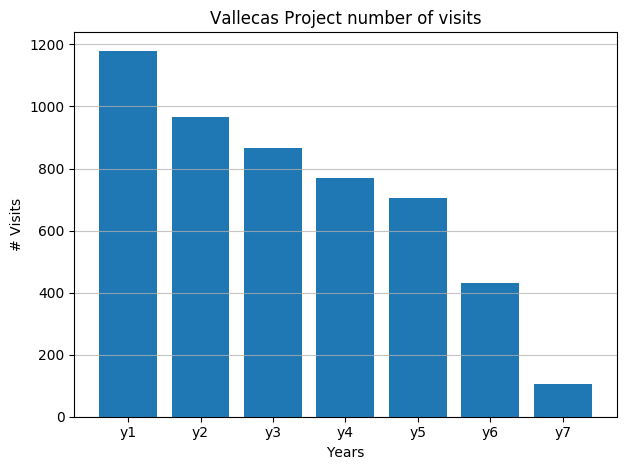
\includegraphics[keepaspectratio, width=0.6\linewidth]{figures/Fig_visits}
        \caption{Number of volunteers across seven years of \emph{Proyecto Vallecas}. As expected, the number of subjects decreases across time. The number of subjects in the year 1 was 1213 of which 33 were removed because were diagnosed with MCI or AD resulting in 1180 subjects recruited to participate in the study in year 1. 965 of the initial 1180 came for a second visit ($18\%$ drop rate), 865 in year 3 ($27\%$ drop rate from year 1), 770 in year 4 ($35\%$ drop rate from year 1), 704 in year 5 ($40\%$ drop rate from year 1), 431 in year 6($63\%$ drop rate from year 1) and 107 in year 7 which at this moment still ongoing ($91\%$ drop rate from year 1). The total number of visits in five years amounts to 5022.} \label{fig:pv5years}
\end{figure}

The structure of the document is as follows. Section \ref{se:int} provides a comprehensive description of the information collected, the description relies upon visual charts and we also study the distribution of some key features collected in \emph{Proyecto Vallecas} dataset.
Section \ref{se:met} shows statistical tests and the correlation analysis paying special attention to the evolution of the longitudinal variables and their underlying relationship with cognitive performance. 
Section \ref{se:met} describes the features that are most strongly related to cognitive decline for both static (measured once) and dynamic variables (measured every year). We extract features from the longitudinal features to build a classifier based on relevant features extracted from time series \cite{christ2018time}. We conclude with the discussion of the results and future works in Section \ref{se:con} connecting our findings with previous populational studies.  

% YS give full description of features
% Description of the dataset table with all features
% draw time line of the prj

%Sleep
%Diet APOE
%'Cardiovascular_s', 'PhysicalExercise_s', 'Sleep_s', 'Anthropometric_s', 'Diet_s', 'SocialEngagement_s', 'TraumaticBrainInjury_s', 'Demographics_s', 'EngagementExternalWorld_s'

\subsection{Exploratory Data Analysis static variables}
\label{sse:eda}
%Static as the correlate with conversion
In this section we perform Exploratory Data Analysis (EDA). The objective of EDA is to build graphical representations that help us make sense of the data. EDA gives us a bird's eye of the dataset aiding at identifying patterns and trends and most importantly, assisting in framing the type of questions we want to ask.
EDA relies upon a careful pre-processing of the dataset. We perform EDA in a succession of steps. We will start with a preliminary data analysis plotting basic information of the dataset such as the age distribution and other demographics of the participants. 
We will also study the distribution of the most significant features of all type of features indicated in Table \ref{tab:vallecasvars}. Furthermore, we plot the distribution of cognitive decline conditional to other features. This will set the stage for the correlation analysis described in Section \ref{se:res} for both static (one observation) and dynamic variables (time series).


% features_dict['Anthropometric_s'] == ['lat_manual', 'pabd', 'peso', 'talla', 'audi', 'visu', 'imc']
% Plot 'pabd', 'peso', 'talla', 'audi'
\subsubsection{Genetic, Anthropometric and Demographic}
\label{ssse:ant}
Figure \ref{fig:apoe} shows the APOE Genotyping test, classifying the subjects in three groups depending on whether they have no copy of the APO$\epsilon4$ allele, one copy APO$\epsilon4$ heterozygotes or two copies of APO$\epsilon4$ \cite{farrer1997effects}. The APO$\epsilon4$ variant is the largest known genetic risk factor for late-onset sporadic Alzheimer's disease (AD). However researchers have observed risk changes of APO$\epsilon4$ presence with factors such as ethnicity. For instance, Nigerian blacks have the highest observed frequency of the APO$\epsilon4$ allele in world populations, but at the same time AD is apparently less frequent in Nigerians than in other populations \cite{sepehrnia1989genetic}.
Estimated worldwide human allele frequencies of ApoE is $13.7\%$ and $36.7\%$ in AD patients. On the other hand, $40–65\%$ of AD patients have at least one copy of the APO$\epsilon4$ allele.

In our population, $82\%$ were APO$\epsilon4$ negative, $17\%$ APO$\epsilon4$ heterozygotes and $1\%$ APO$\epsilon4$ homozygotes. 
%DO p(AD|+ in apoe)

\begin{figure}[H]
        \centering
        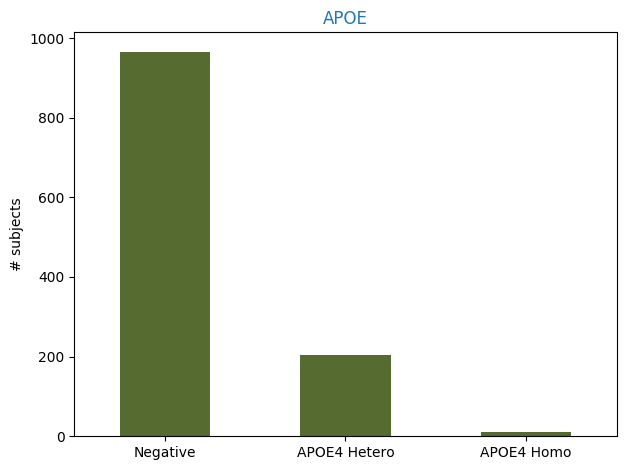
\includegraphics[keepaspectratio, width=0.6\linewidth]{figures/Fig_apoe}
        \caption{APOE Genotyping testing in \emph{Proyecto Vallecas} dataset. $17\%$ of subjects carry at least one copy of the $\epsilon4$, slightly higher than the worldwide estimates in Caucasian population ($13.7\%$) indicated in \cite{farrer1997effects}} 
        \label{fig:apoe}
\end{figure}

Figure \ref{fig:anthro} shows the histogram for anthropometric variables bmi, abdominal perimeter, weight and height, measured at year 1.
\begin{figure}[H]
        \centering
        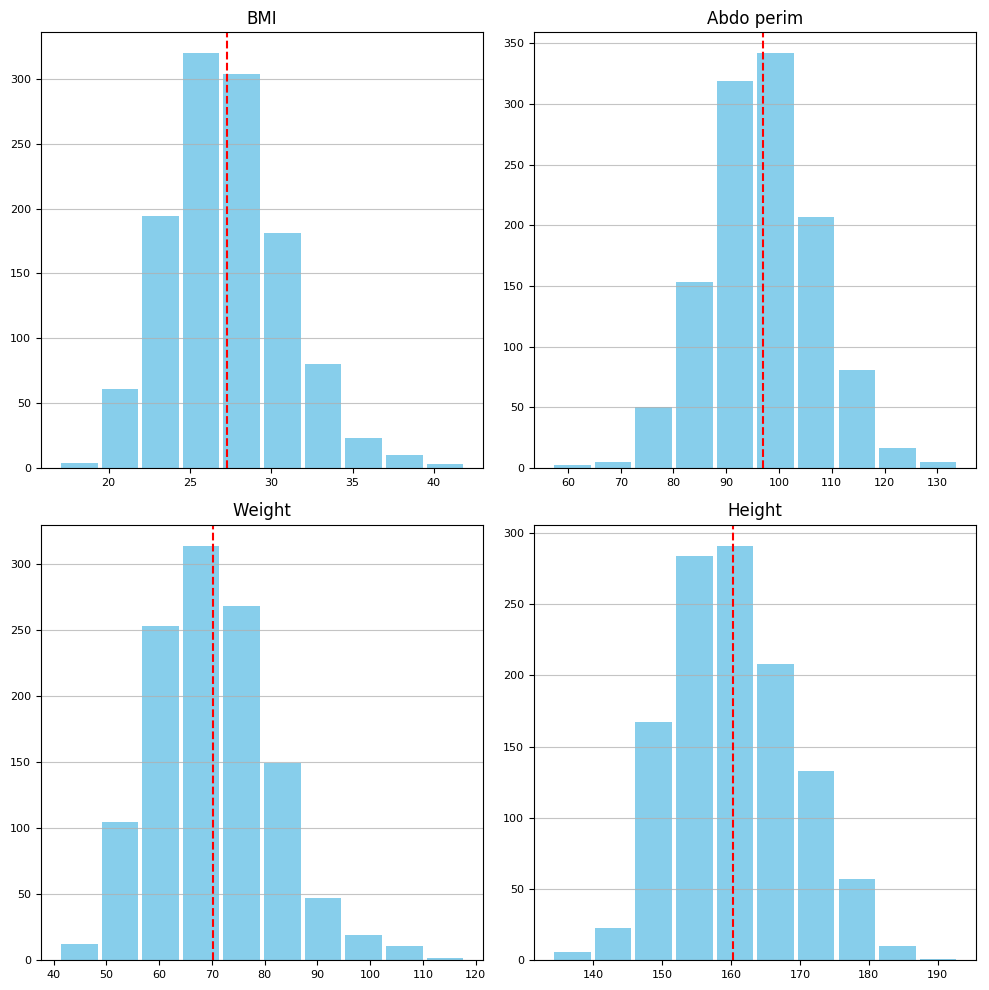
\includegraphics[keepaspectratio, width=.8\linewidth]{figures/Fig_anthro}
        \caption{Histogram of anthropometric variables measured in year 1 of \emph{Proyecto Vallecas} dataset. Clockwise, Body Mass Index (min=16.95, max=41.93), abdominal perimeter (min=57cm, max=134cm), weight (min=41kg, max=118kg) and height(min=134cm, max=193cm)} 
        \label{fig:anthro}
\end{figure}

Figure \ref{fig:sexlat} shows the histogram for sex and hand laterality.
%Change this figure
\begin{figure}[H]
        \centering
        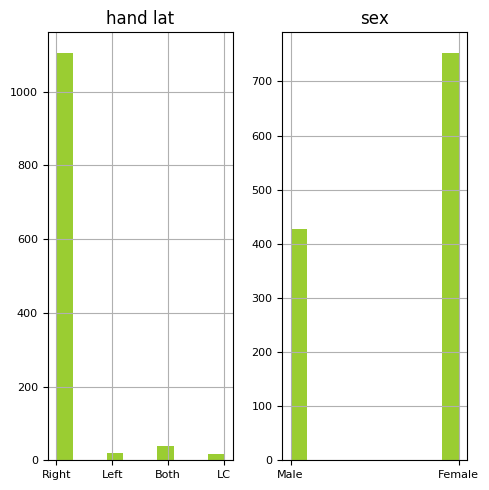
\includegraphics[keepaspectratio, width=.4\linewidth]{figures/Fig_sexlat}
        \caption{Histogram of hand laterality (left) and sex (right). There is majority of females, 753 versus 427 males. The right handed are 1106, left 19, ambidextrous 39 and 16 were forced right abut born left.} 
        \label{fig:sexlat}
\end{figure}

% features_dict['Demographics_s'] == ['edad', 'edad_visita7']
Figure \ref{fig:ages} shows ages of participants at the inception of the project and the age of the participants that came to the seventh visit.

\begin{figure}[H]
        \centering
        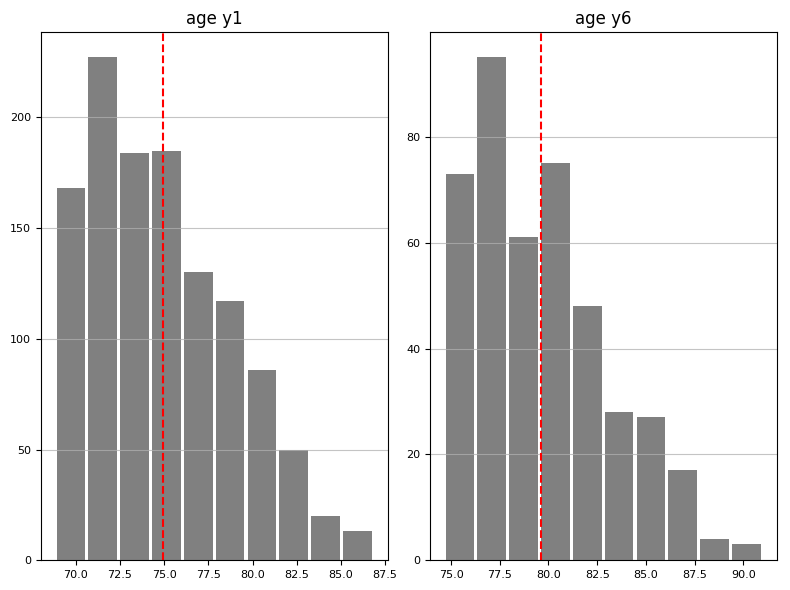
\includegraphics[keepaspectratio, width=.6\linewidth]{figures/Fig_ages}
        \caption{Histogram of the age of the participants in the first and last years of the \emph{Proyecto Vallecas} dataset. The youngest and the oldest participant in year 1 were 69 and 86 years old respectively. In year 7 the minimum and maximum ages are 76 and 89.} 
        \label{fig:ages}
\end{figure}

%['renta', 'nivelrenta', 'educrenta', 'municipio', 'barrio', 'distrito', 'sexo', 'nivel_educativo', 'anos_escolaridad', 'familial_ad', 'sdestciv', 'sdhijos', 'numhij', 'sdvive', 'sdocupac', 'sdresid', 'sdtrabaja', 'sdeconom', 'sdatrb']

Figure \ref{fig:incomeresidency} shows the home residency and the income distribution of \emph{Proyecto Vallecas} subjects as estimated based on their home residency. A more in detail representation of the home residency is shown in figure \ref{fig:resid_detail}

\begin{figure}[H]
        \centering
        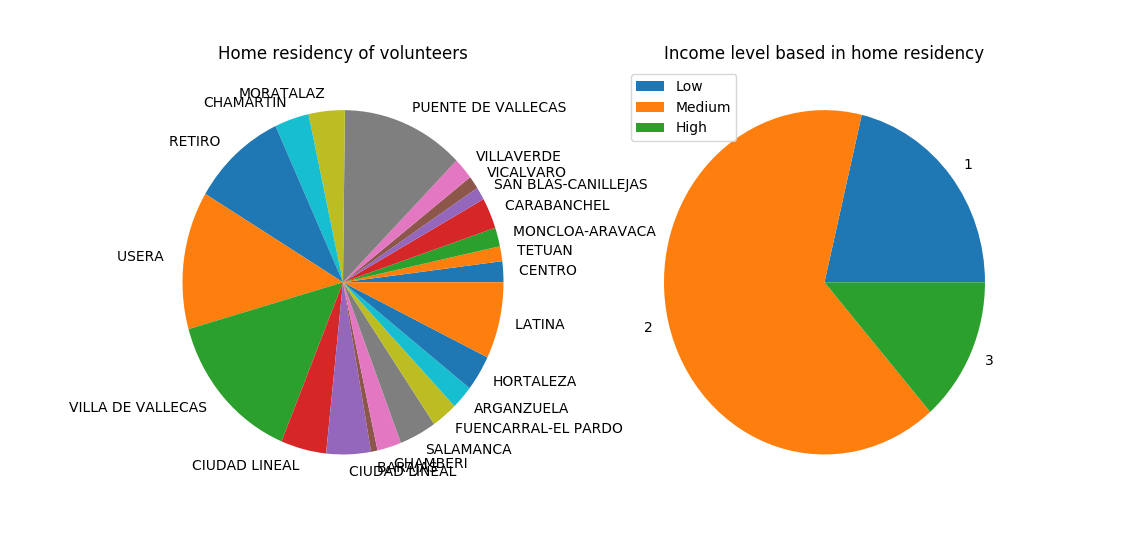
\includegraphics[keepaspectratio, width=.8\linewidth]{figures/incomeresidency}
        \caption{On the left, distribution of home residency by districts of \emph{Proyecto Vallecas} volunteers. All districts of the city of Madrid are represented. Note that there are 156 subjects of a total of 1180 that are not residents in the city of Madrid and are not included here. On the right, we plot the income distribution as estimated based on the home residency, 251 subjects live in low income areas, 769 in medium income areas and 160 in high income neighborhoods of Madrid.
        } \label{fig:incomeresidency}
\end{figure}

% Create figure and dsave it properly as png
% \begin{figure}[]
%         \centering
%         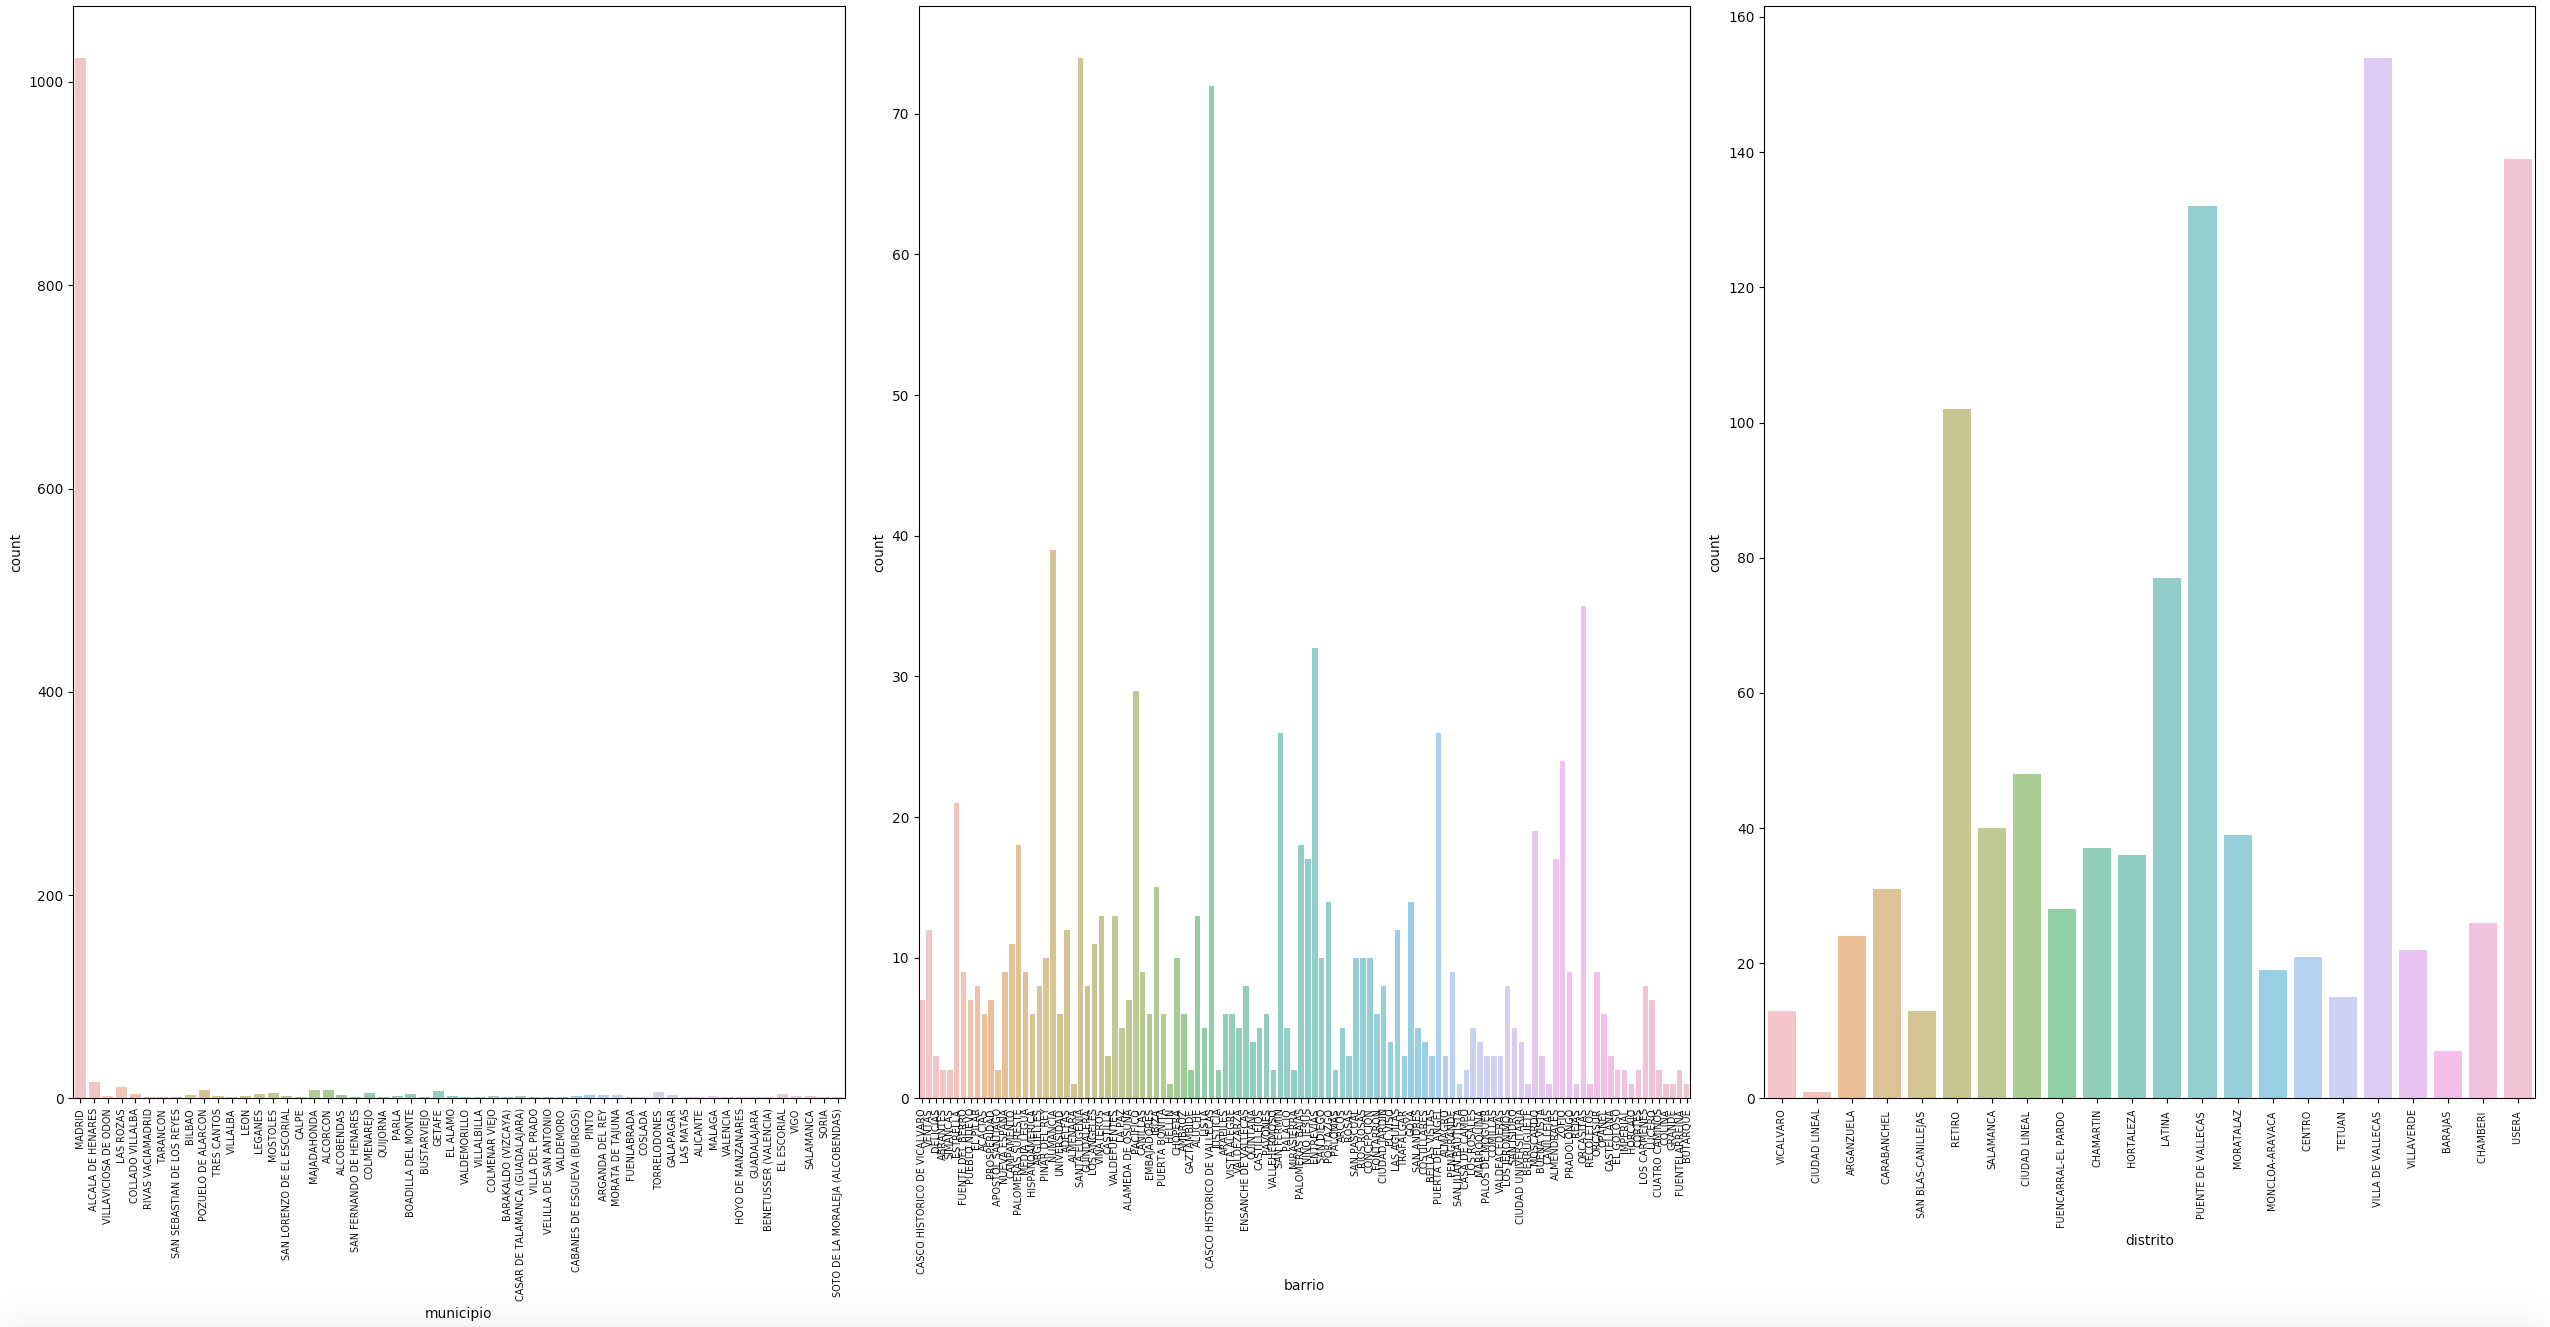
\includegraphics[height=\textheight, width=\textwidth]{figures/resid_detail}
%         \caption{On the left, city of residency of subjects, the large majority lives in Madrid. Middle figure neighborhood and right figure borough of residence in the city of Madrid. 
%         } \label{fig:incomeresidency}
% \end{figure}

Figure \ref{fig:demo} depicts the rest of demographic variables including: educational attainment, number of sons, years of work as an employee, self-assessed economic status, marital status and the number of people living at home.
\begin{figure}[H]
        \centering
        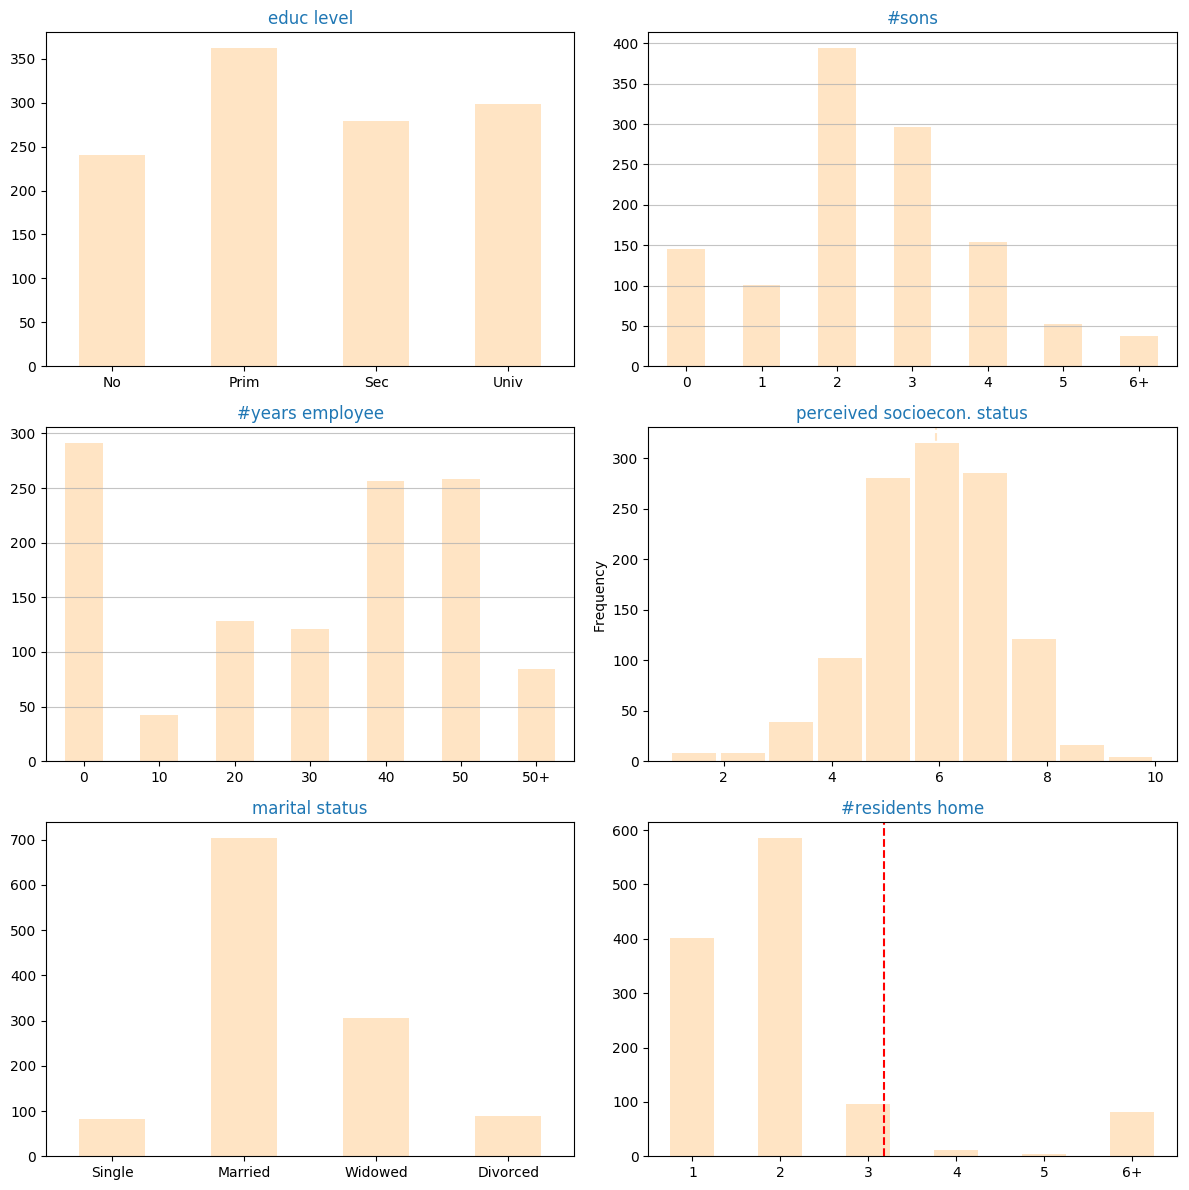
\includegraphics[keepaspectratio, width=\linewidth]{figures/Fig_demo}
        \caption{Histogram of demographic variables in the \emph{Proyecto Vallecas} dataset measured in the first year. Clockwise, educational attainment classified as \emph{no formal education, primary school, secondary school and university degree}, number of sons, number of years of work as an employee, self-assessed economic status (1 the lowest, 10 the highest, marital status (\emph{single, married, widows, divorced}) and the number of people living at home.} 
        \label{fig:demo}
\end{figure}

\subsubsection{Sleep}
\label{ssse:sleep}

Figure \ref{fig:sleep} depicts features related to sleep patterns of the subjects. Daily naps are less common that what it could be expected from a Spaniard population aged 70 or more. $37\%$ of subjects do not take any nap at all, $24\%$ of subjects sleep daily between 15 and 30 minutes and the $17$ report to take naps of at least one hour a day. The majority of subjects report remembering their dreams $67.7\%$ versus $32\%$ that do not. The majority of subjects report to snore during sleep $60\%$. 
% YS remove TBI of charts
\begin{figure}[H]
        \centering
        \includegraphics[keepaspectratio, width=\linewidth]{figures/Fig_sleep}
        \caption{Histogram of sleep variables in the \emph{Proyecto Vallecas} dataset in the first year. From left to right and up to the bottom, number of hours of sleep during the day ($\mu=0.45, \sigma=1$), tingling during sleep (0 No, 1 Yes, 9 Dk/Da), movements during sleep (0 No, 1 Yes, 9 Dk/Da), number of hours of night sleep ($\mu=6.8, \sigma=1.3$), deep sleep (1 Light, 2 Moderate, 3 Deep), remember dreams (0 No, 1 Yes, 9 Dk/Da), snoring (0 No, 1 Yes, 2 snore and difficult breathing 9 Dk/Da), noises during sleep (0 No, 1 Yes, 9 Dk/Da), sufficient sleep (0 No, 1 Yes, 9 Dk/Da).} 
        \label{fig:sleep}
\end{figure}


\subsubsection{Life style}
\label{ssse:life}
% Food
Figure \ref{fig:food} depicts the type of food consumption as reported by the subjects. $84\%$ of subjects report to consume olive oil $6/7$ days a week, $74\%$ bread, $44\%$ vegetables and $29\%$ report consuming sweets 6/7 days a week.

\begin{figure}[H]
        \centering
        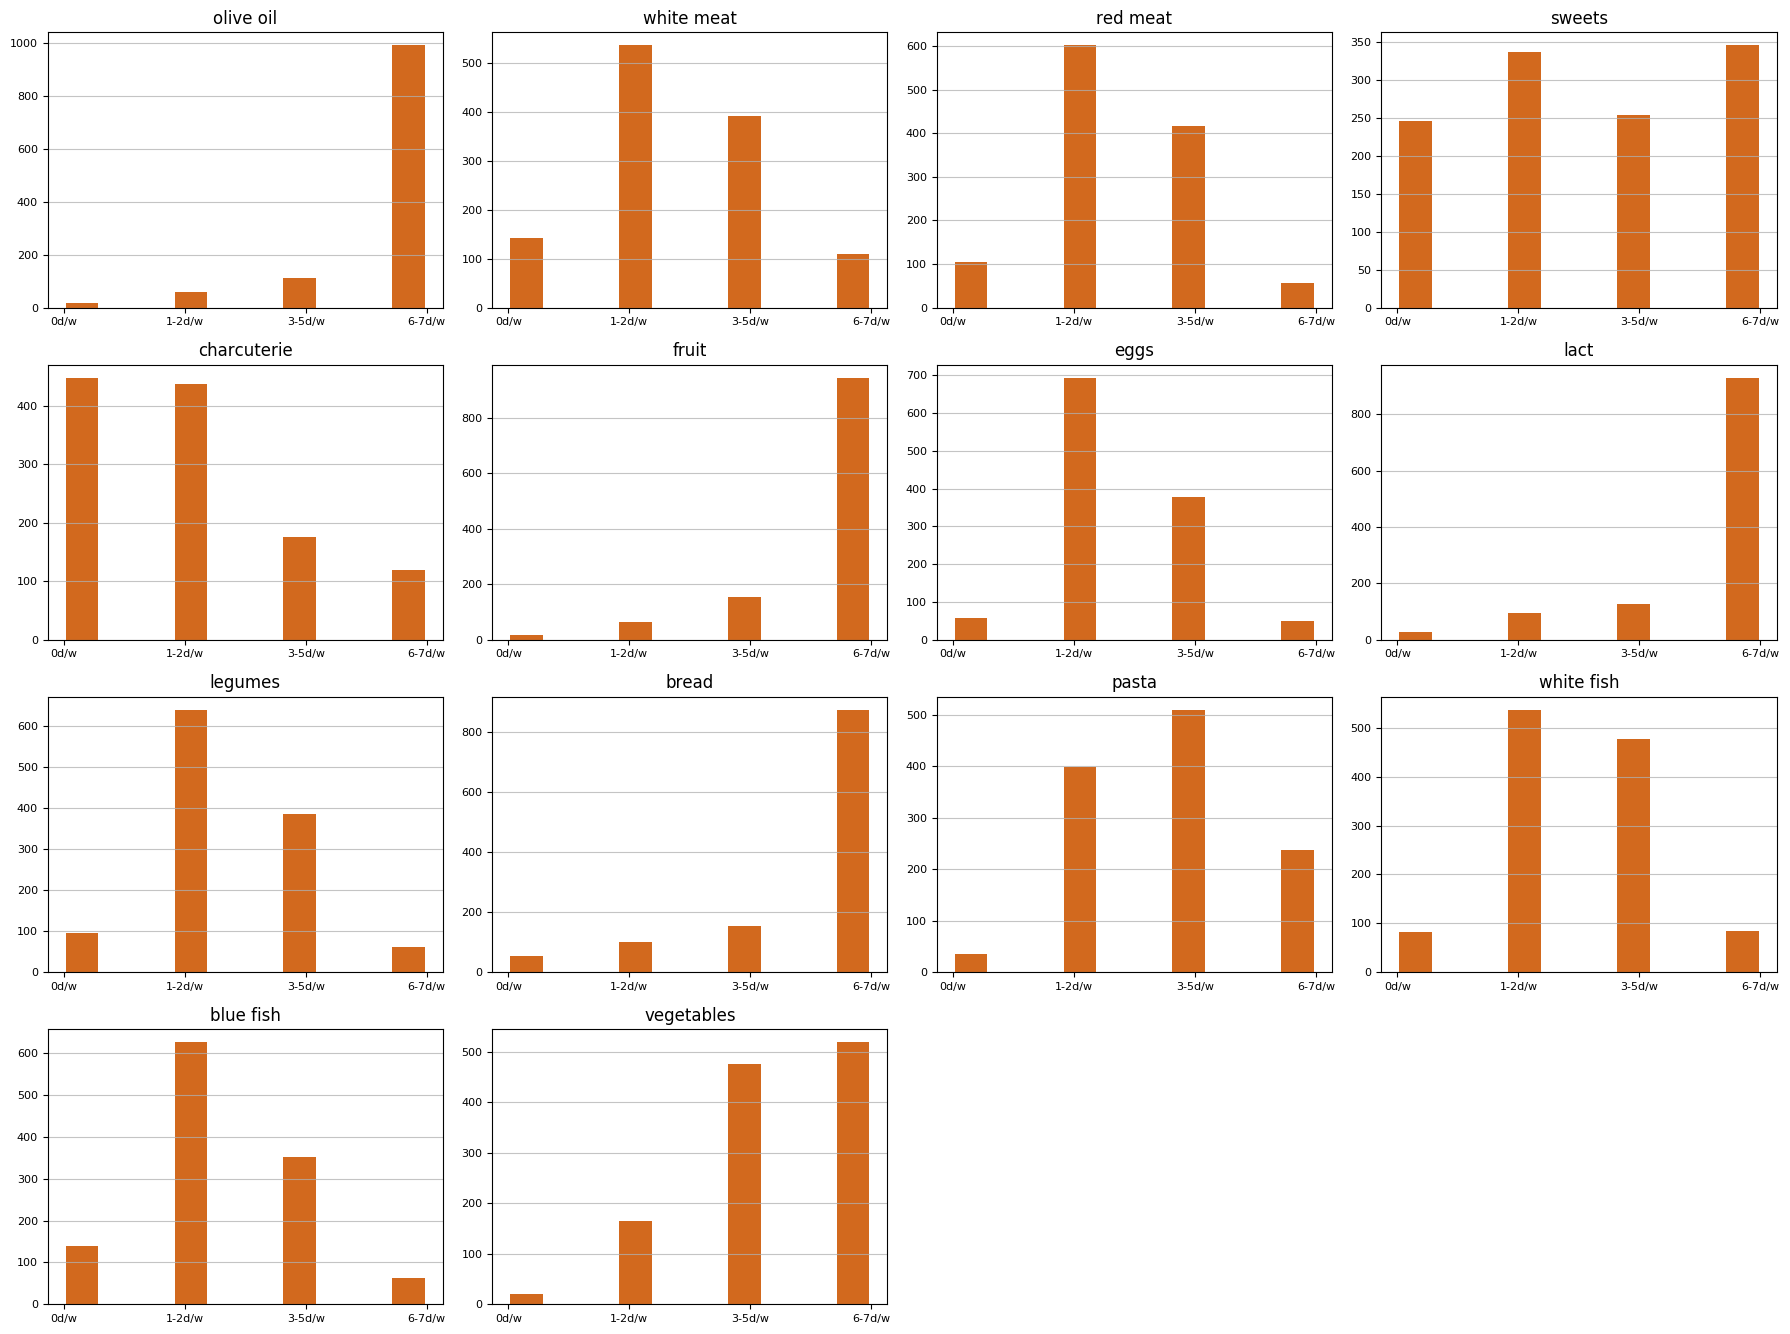
\includegraphics[keepaspectratio, width=\linewidth]{figures/Fig_food}
        \caption{Histogram of type of weekly food consumption reported by the subjects in the first visit. The x-axis of each chart represents how many days a week they consume which type of food. The large majority of subjects report a daily consumption of bread, milk and olive oil.}
        \label{fig:food}
\end{figure}

%Diet
Figure \ref{fig:diet} depicts the type diet estimated based on the reported weekly food consumption. We distinguish between three different diets: strong glucemic component(carbs, sweets), strong proteic component (red meat, eggs, fish) and Mediterranean (fruit, fish, vegetables) and we calculate an score for each diet based on REF-MA.

\begin{figure}[H]
        \centering
        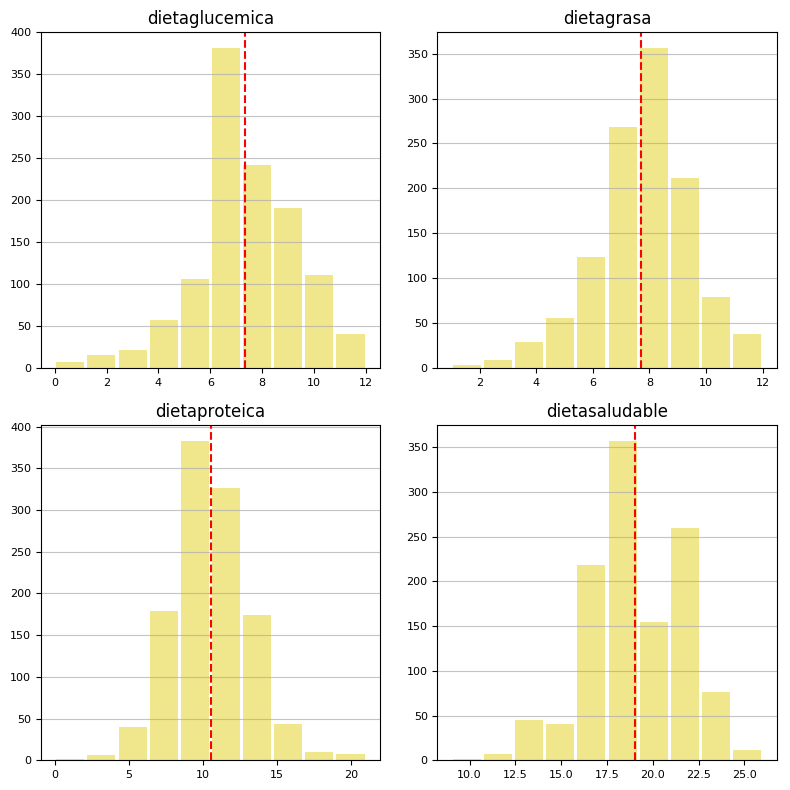
\includegraphics[keepaspectratio, width=.8\linewidth]{figures/Fig_diet}
        \caption{Histogram of type of diet based on weekly food consumption as reported by the subjects in the first visit. The x-axis of each chart represents the score for each type of diet, the larger the score the most prevalent the main component of the diet is in the subject's diet. For example, a subject with a score of 12 in the glucemic diet will likely consume more sweets than a subject a score of 6, by the same token a subject with a large score in the Mediterranean diet will likely consume more fruit and vegetables than a subject with a lower score.} 
        \label{fig:diet}
\end{figure}

Obesity (Higher midlife BMI) is related to higher risk of dementia and AD, independently of obesity-related risk factors and co-morbidities \cite{tolppanen2014midlife}, \cite{nepal2014rising}. 

The distribution of the BMI in our population is particularly interesting $(\mu_{BMI}=27.3, \sigma_{BMI}=3.6)$. $26.8\%$ of the population have healthy weight ($BMI \in [18.5, 25]$), $51.8\%$ have over weight ($BMI \in [25,30]$) and $21.4\%$ are obese ($BMI > 30$). 
The majority of subjects report to have hypertension $53\%$ vs $47\%$, this in line with larger studies 28,887 participants in Spain aged 35-74, high blood pressure was present in $47\%$ in men and $39\%$ in women) \cite{grau2011cardiovascular}, \cite{lacruz2015prevalence}.
$27\%$ of the participants declared to be smokers and $33\%$ ex-smokers.

 %total cholesterol ≥ 250 mg/dL (43% and 40%, respectively), 
 %obesity (29% and 29%, respectively), tobacco use (33% and 21%, respectively), and diabetes (16% and 11%, respectively). Total cholesterol ≥ 190 and ≥ 250 mg/dL were the respective minimum and maximum coefficients of variation (7%-24% in men, 7%-26% in women). Average concordance in lipid measurements between laboratories was excellent. 
%of note the self reported hypertension is inferior to population studies in which the blood pressure is actually measured mean systolic $\geq140$ mmHg and/or diastolic BP (DBP) $\geq90$ mmHg and/or use of antihypertensive medication \cite{lacruz2015prevalence}. 

%https://www.brightfocus.org/alzheimers/article/weight-risk-factor-alzheimers-disease

%https://www.isglobal.org/en/new/-/asset_publisher/JZ9fGljXnWpI/content/cardiopatia-isquemica-demencias-e-ictus-se-situan-como-las-principales-causas-de-muerte-en-espana

%YS: change arrythmia in pic for stroke 3 top
\begin{figure}[H]
        \centering
        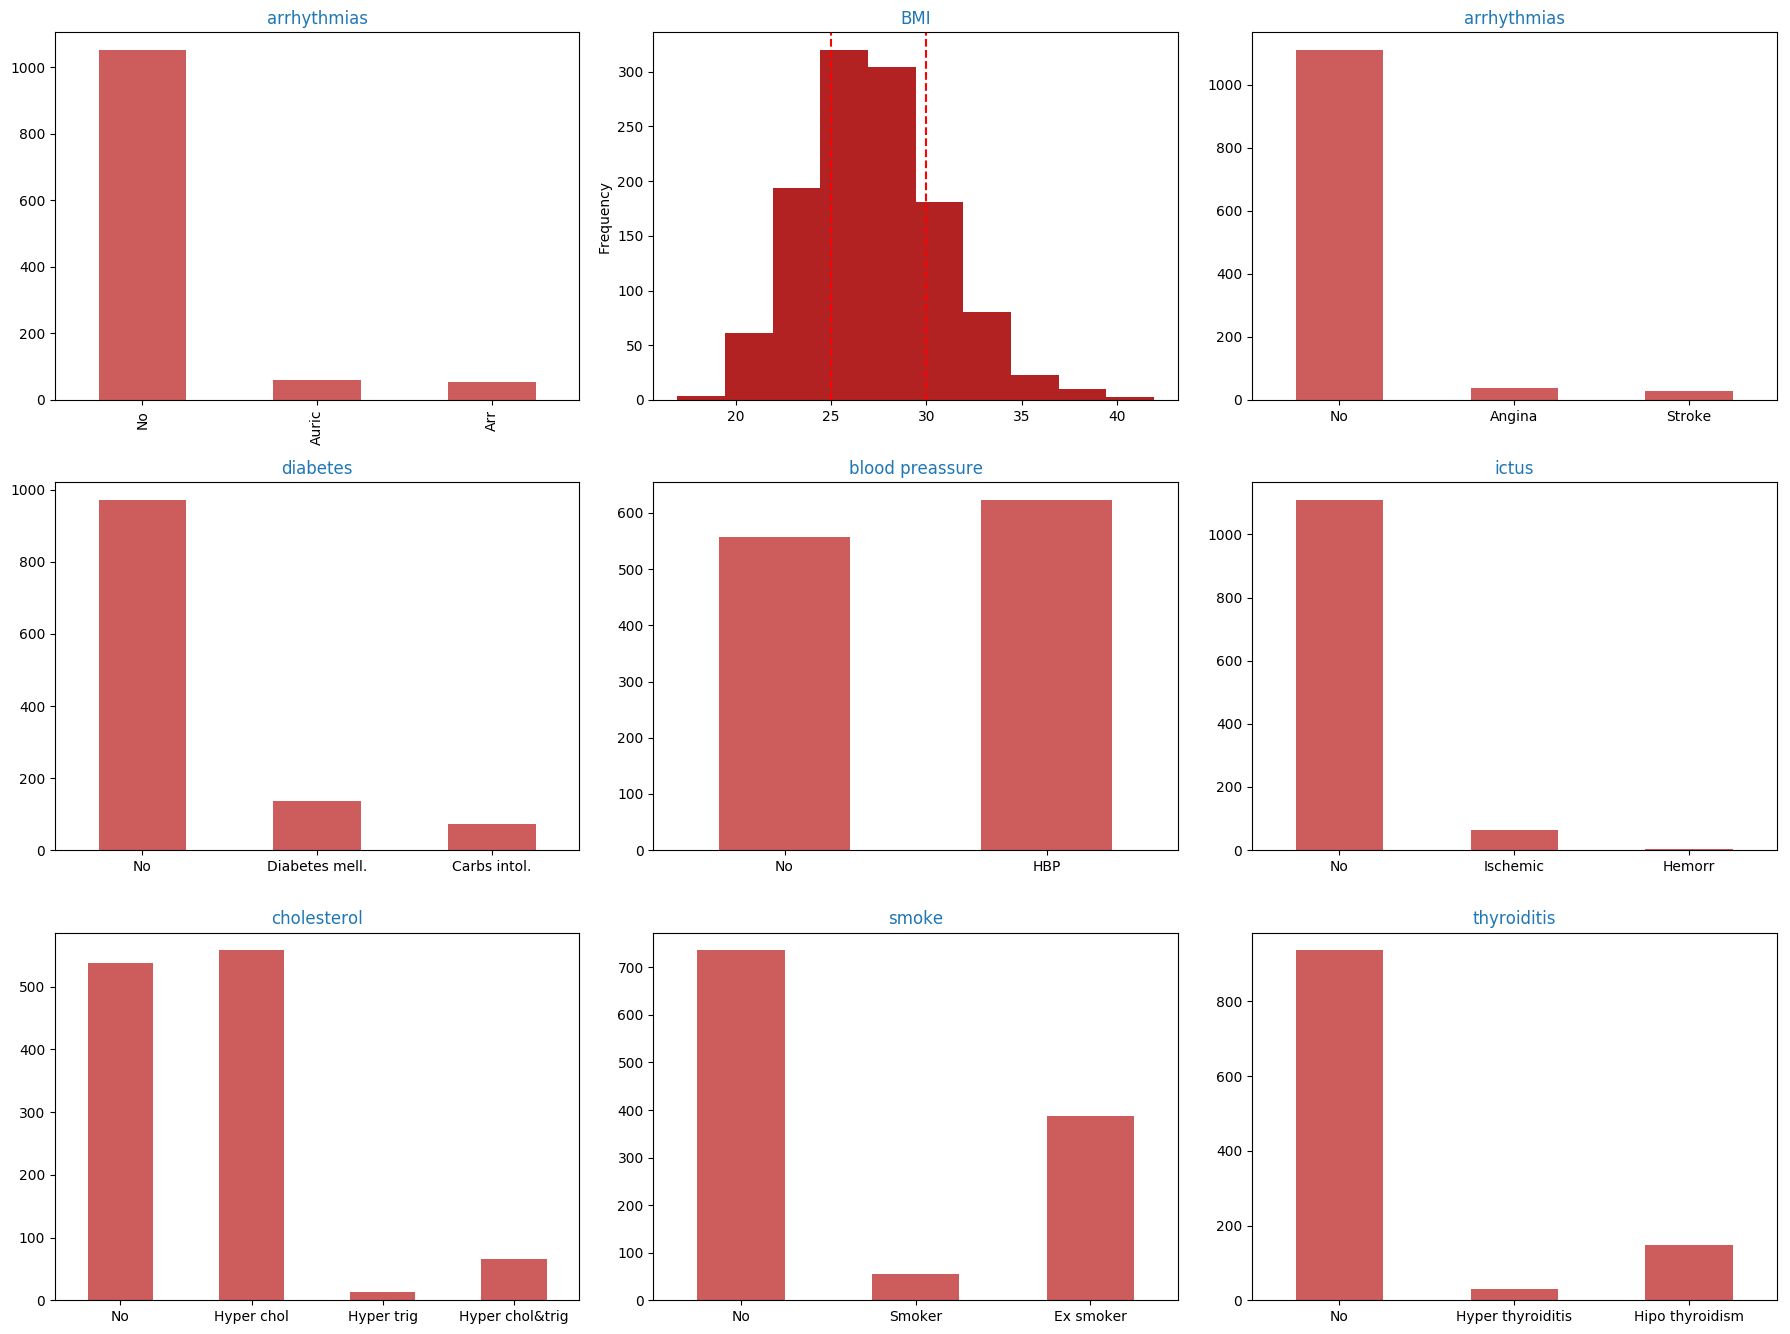
\includegraphics[keepaspectratio, width=\linewidth]{figures/Fig_cardio}
        \caption{Histogram of features related to cardiovascular health. From top down and left to right: arrythmias (\emph{No Arrhythmia, Atrial fibrillation, Arrhythmia}), body mass index, heart stroke (\emph{No past strokes, Angina, Stroke}), diabetes (\emph{No diabetic, diabetes mellitus, intollerance to carbs}), hypertension, ictus historial (\emph{No, Ischemic, Hemorrhagic}), cholesterol (\emph{No cholesterol, hyper cholesterol, Hyper triglycerides, both hyper cholesterol and triglycerides}), Smoke (\emph{Non smoker, Smoker, Ex-smoker}), thyroiditis (\emph{No thyroiditis, Hyper thyroiditis, hipo thyroiditis}). } 
        \label{fig:cardio}
\end{figure}

%PhysicalExercise_s ['ejfre', 'ejminut']
%YS: fig left, cambio 1,2 por dias a la semana
Figure \ref{fig:phys} depicts features related to physical exercise. The subjects were asked the frequency in days per week of their physical exercise and the duration of the sessions.
\begin{figure}[H]
        \centering
        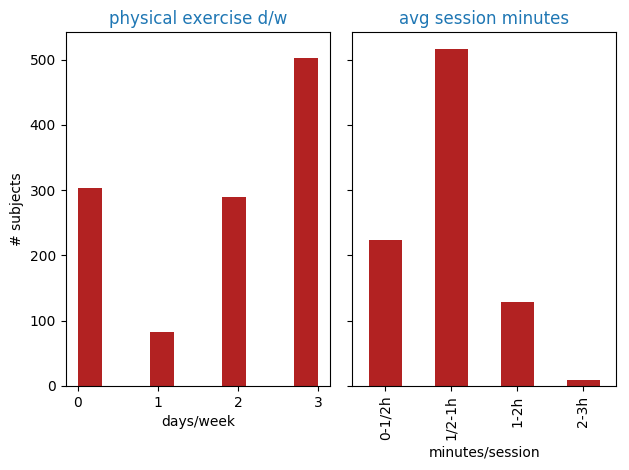
\includegraphics[keepaspectratio, width=0.6\linewidth]{figures/Fig_phys}
        \caption{Histogram of features related to physical exercise. On the left days/week that subjects report to practice physical exercise, and on the right the average duration of the sessions (\emph{less than 30 minutes, less than one hour, between one and tow hours, more than two hours})} 
        \label{fig:phys}
\end{figure}

%EngagementExternalWorld_s ['a01', 'a02', 'a03', 'a04', 'a05', 'a06', 'a07', 'a08', 'a09', 'a10', 'a11', 'a12', 'a13', 'a14']

Figure \ref{fig:engage} depicts features related to engagement with the external world of the subject. In particular, doing creative activities, going out with friends, travel and tourism, community activities (e.g. cultural associations and NGO), going to church, visit social club, go to the movie theater or art shows, go to sport events, how often listens to music, how often watches/listens TV/radio, reading habits (books, newspaper, magazines), and use of the internet and IT.
%EngagementExternalWorld_s ['a03' amigos, 'a04' travel, 'a05' ong, 'a06' church, 'a08' cine, 'a09' sport, 'a10' music, 'a11' tv, 'a12' read, 'a13' internet] 
Of interest, church goers are a minority in our population, $75\%$ never go to church, $17\%$ that go a few times and $8\%$ go often. $86\%$ habitually watches the TV or listens to the radio, $68\%$ read books or magazines often and only $29\%$ use the Internet often.

\begin{figure}[H]
        \centering
        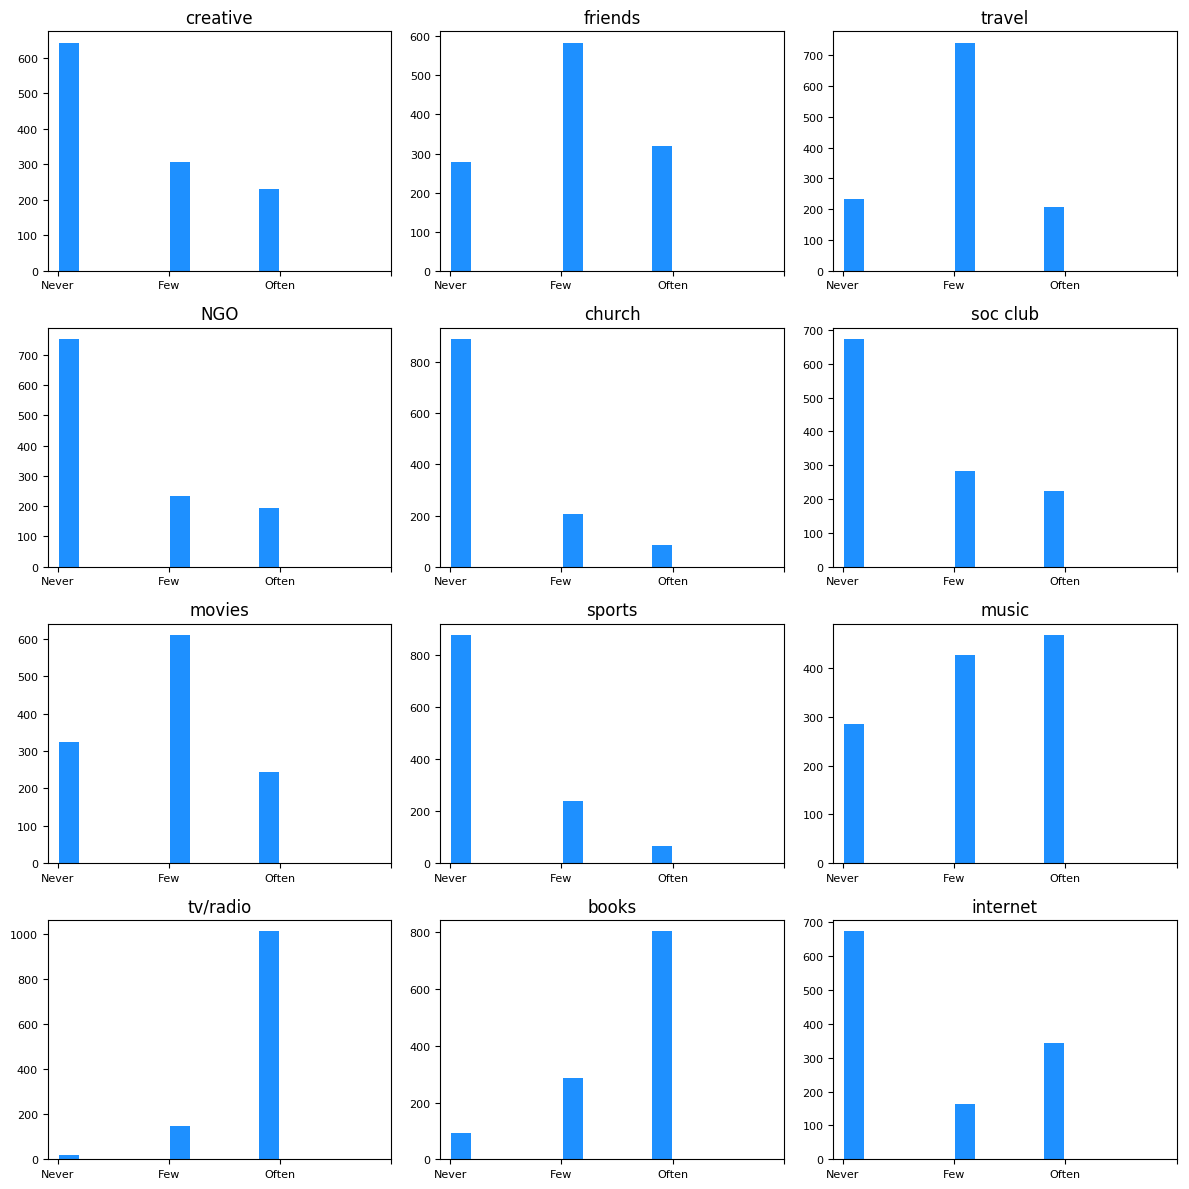
\includegraphics[keepaspectratio, width=\linewidth]{figures/Fig_engage}
        \caption{Histogram of features that reflect engagement with the external world from the part of the subject. From top down and left to right the charts depict the number of subjects that get involve in creative activities, going out with friends, travel and tourism, community activities (e.g. cultural associations and NGO), going to church, visit social club, go to the movie theater or art shows, go to sport events, how often listens to music, how often watches/listens TVradio , how often reads (books, newspaper, magazines), how often uses the internet.} 
        \label{fig:engage}
\end{figure}

\subsubsection{Cardiovascular}
\label{ssse:cardio}

% Cardiovascular_s ['hta', 'hta_ini', 'glu', 'lipid', 'tabac', 'tabac_cant', 'tabac_fin', 'tabac_ini', 'sp', 'cor', 'cor_ini', 'arri', 'arri_ini', 'card', 'card_ini', 'tir', 'ictus', 'ictus_num', 'ictus_ini', 'ictus_secu']
Figure \ref{fig:cardio} depicts features related to the cardiovascular health self reported in our population. The subjects were asked whether they suffer hypertension, angina and heart attack, glucose metabolism disorders, dyslipidemia (an abnormal amount of lipids in the blood), arrhythmias, and if they smoke. 
Thyroid hormones have a significant impact on cardiac function and structure (excess thyroid hormone affects cardiovascular \cite{klein2007thyroid}), subjects also reported whether they suffer from hyper(hipo)thyroidism.
Stroke is a risk factor for coronary heart disease and subjects were asked if they had in the past hemorrhagic or ischemic cerebral ictus. Ischemic stroke and AD share pathophysiological mechanisms such as inflammation, immune exhaustion and neurovascular damage \cite{lucke2015common}. 
The causality between AD and hemorrhagic stroke seems to be reversed (AD causes X, rather than the usual search of factor X that causes AD), patients who had Alzheimer's disease are at the highest risk of hemorrhagic stroke \cite{wang2014newly}.
% Pass on sp (you think you are overweighted?) and use If your BMI is 25.0 to <30, it falls within the overweight range. If your BMI is 30.0 or higher, it falls within the obese range

\subsubsection{Traumatic brain injury}
\label{ssse:tbe}
%TraumaticBrainInjury_s ['tce', 'tce_con', 'tce_ini', 'tce_num', 'tce_secu']
Figure \ref{fig:tce} shows the distribution of episodes (at least one) of traumatic brain injury. 
\begin{figure}[H]
        \centering
        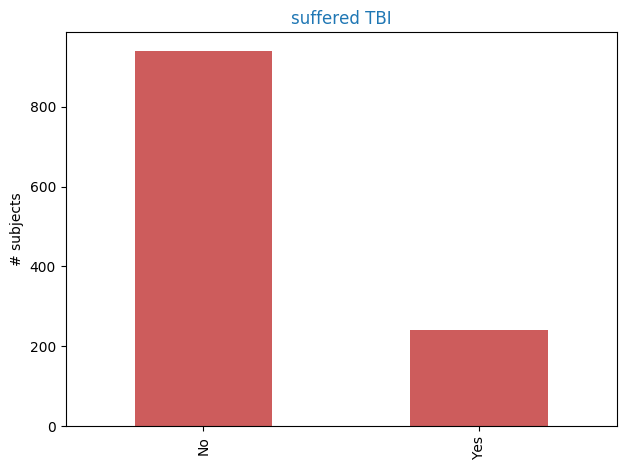
\includegraphics[keepaspectratio, width=0.6\linewidth]{figures/Fig_tce}
        \caption{Histogram of traumatic brain injury. $20\%$ of subjects declared to have suffered in the past an episode of traumatic brain injury of unspecified seriousness.} 
        \label{fig:tce}
\end{figure}


\subsection{Exploratory Data Analysis longitudinal variables}
\label{se:eda_long}
%'CognitivePerformance', 'Diagnoses', 'Neuropsychiatric', 'QualityOfLife', 'Genetics_s', 'SCD', 'Demographics', 'Cardiovascular_s', 'PhysicalExercise_s', 'Sleep_s', 'Anthropometric_s', 'Diet_s', 'SocialEngagement_s', 'TraumaticBrainInjury_s', 'Demographics_s', 'EngagementExternalWorld_s'
The longitudinal variables are MRI, cognitive performance, Neuropsychiatric, QualityOfLife, and SCD.
\subsubsection{MRI}
\label{sse:mri}


\subsubsection{Cognitive Performance}
\label{sse:cogper}
Figures \ref{fig:cogperyears} and \ref{fig:cogperyears} plot the evolution of four measures related to cognitive performance. Figure \ref{fig:cogperyears}, clockwise and starting in the top left chart: score for the number of words that start by the letter p in one minute, score for the number of animals that the subject can recall in one minute, score of speed processing of symbols and the score in the mini-mental examination (MMSE). 

\begin{figure}[H]
    \centering
    \begin{subfigure}[t]{0.4\textwidth}
        \centering
        \includegraphics[height=2.1in]{figures/p_visita}
        \caption{Histograms of number of words that start by the letter p for each year.}
    \end{subfigure}
    \hfill
    \begin{subfigure}[t]{0.4\textwidth}
        \centering
        \includegraphics[height=2.1in]{figures/animales_visita}
        \caption{Histograms of number of animals recalled each year.}
    \end{subfigure}%\quad
    
     \begin{subfigure}[t]{0.4\textwidth}
        \centering
        \includegraphics[height=2.1in]{figures/cn_visita}
        \caption{Histograms of score of speed processing of symbols for each year.}
    \end{subfigure}
    \hfill
    \begin{subfigure}[t]{0.4\textwidth}
        \centering
        \includegraphics[height=2.1in]{figures/mmse_visita}
        \caption{Histograms of score of the MMSE test score for each year.}
    \end{subfigure}%\quad
   
    \caption{Histograms showing the evolution of features related to the cognitive performance of the subjects across the seven years of \emph{Vallecas Project}. From left to right and top to bottom: number of words that start by letter p, number of animals, speed processing of symbols and MMSE.}
    \label{fig:cogperyears}
\end{figure}

Figure \ref{fig:cogper4} plots the time series for four measures related to cognitive performance. Clockwise starting top left chart: score of speed processing of symbols, score for the number of animals that the subject can recall in one minute, score for the number of words that start by the letter p in one minute and the score in the mini-mental examination (MMSE).

\begin{figure}[H]
    \centering
    \begin{subfigure}[t]{0.45\textwidth}
        \centering
        \includegraphics[height=2.5in]{figures/p_visita1_years}
        \caption{Time series (indexed in years) of the  number of words that start by the letter p that subjects can recall in one minute. The statistics for years 1 to 5 (years 6 and 7 are still ongoing): $\mu_{1}=13.44, \sigma_{1}=7.02$, $\mu_{2}=14.16, \sigma_{2}=4.96$, $\mu_{3}=14.30, \sigma_{3}=4.94$, $\mu_{4}=14.21, \sigma_{4}=4.94$,$\mu_{5}=14.71,\sigma_{5}=4.92$.}
    \end{subfigure}
    \hfill
    \begin{subfigure}[t]{0.45\textwidth}
        \centering
        \includegraphics[height=2.5in]{figures/animales_visita1_years}
        \caption{Time series the  number of animals that subjects can recall in one minute. The statistics for years 1 to 5 (years 6 and 7 are still ongoing): $\mu_{1}=18.21, \sigma_{1}=8.71$, $\mu_{2}=17.76, \sigma_{2}=5.12$, $\mu_{3}=18.48, \sigma_{3}=5.40$, $\mu_{4}=18.29, \sigma_{4}=5.54$,$\mu_{5}=18.32,\sigma_{5}=5.50$.}
    \end{subfigure}%\quad
    
     \begin{subfigure}[t]{0.45\textwidth}
        \centering
        \includegraphics[height=2.5in]{figures/cn_visita1_years}
        \caption{Time series of feature \emph{cn} which measures the speed processing of symbols in a task (attention and velocity). This measure tends to be more stable than other eg Buschke. The statistics for years 1 to 5 (years 6 and 7 are still ongoing): $\mu_{1}=18.71, \sigma_{1}=7.60$, $\mu_{2}=18.70, \sigma_{2}=7.47$, $\mu_{3}=18.81, \sigma_{3}=7.55$, $\mu_{4}=18.54, \sigma_{4}=7.67$,$\mu_{5}=18.05,\sigma_{5}=7.35$.}
    \end{subfigure}
    \hfill
    \begin{subfigure}[t]{0.45\textwidth}
        \centering
        \includegraphics[height=2.5in]{figures/mmse_visita1_years}
        \caption{Time series of the score of the minimental examination test MMSE. The statistics for years 1 to 5 (years 6 and 7 are still ongoing): $\mu_{1}=28.40, \sigma_{1}=1.78$, $\mu_{2}=28.44, \sigma_{2}=1.80$, $\mu_{3}=28.23, \sigma_{3}=2.00$, $\mu_{4}=28.11, \sigma_{4}=2.28$,$\mu_{5}=27.94,\sigma_{5}=2.45$.}
    \end{subfigure}%\quad
   
    \caption{Time series of cognitive performance across the seven years of \emph{Vallecas Project} of features related to cognitive performance. The x-axis are years from year 1 to year 7 and the y-axis the score. Each plot represents the mean (bold line) and the dispersion or standard deviation (shaded region) across the seven years of \emph{Vallecas Project}.}
    \label{fig:cogper4}
\end{figure}


Figure \ref{fig:cogperyearsbus}, clockwise and starting in the top left chart: Buschke delayed recalled score, mean, sum and the Buschke Integral score which is explained in a forthcoming paper. We address the reader to the Appendix section for more details \ref{}).

\begin{figure}[H]
    \centering
    \begin{subfigure}[t]{0.4\textwidth}
        \centering
        \includegraphics[height=2.1in]{figures/fcsrtlibdem_visita}
        \caption{Histograms of the Buschke delayed recall score for each year.}
    \end{subfigure}
    \hfill
    \begin{subfigure}[t]{0.4\textwidth}
        \centering
        \includegraphics[height=2.1in]{figures/bus_meana_visita}
        \caption{Histograms of of the Buschke arithmetic mean for each year.}
    \end{subfigure}%\quad
    
     \begin{subfigure}[t]{0.4\textwidth}
        \centering
        \includegraphics[height=2.1in]{figures/bus_sum_visita}
        \caption{Histograms of of the Buschke sum for each year.}
    \end{subfigure}
    \hfill
    \begin{subfigure}[t]{0.4\textwidth}
        \centering
        \includegraphics[height=2.1in]{figures/bus_int_visita}
        \caption{Histograms of of the \emph{Buschke Integral} score for each year..}
    \end{subfigure}%\quad
   
    \caption{THistograms showing the evolution of features related to the cognitive performance of the subjects across the seven years of \emph{Vallecas Project}. From left to right and top to bottom: 
    Buschke delayed recall score,Buschke arithmetic mean,  Buschke sum and \emph{Buschke Integral}.}
    \label{fig:cogperyearsbus}
\end{figure}


Figure \ref{fig:busper4} plots the time series for four measures related to cognitive performance measured using the Buschke test. Clockwise starting top left chart: delayed recalled score, mean, sum and the Buschke Integral score which is explained in a forthcoming paper. We address the reader to the Appendix section for more details \ref{}).

\begin{figure}[H]
    \centering
    \begin{subfigure}[t]{0.45\textwidth}
        \centering
        \includegraphics[height=2.5in]{figures/fcsrtlibdem_visita1_years}
        \caption{Time series (indexed in years) of Buscke recall delayed score. The statistics for years 1 to 5 (years 6 and 7 are still ongoing): $\mu_{1}=9.02, \sigma_{1}=3.01$, $\mu_{2}=9.44, \sigma_{2}=3.02$, $\mu_{3}=10.10, \sigma_{3}=3.23$, $\mu_{4}=10.44, \sigma_{4}=3.52$,$\mu_{5}=14.76,\sigma_{5}=3.62$.}
    \end{subfigure}
    \hfill
    \begin{subfigure}[t]{0.45\textwidth}
        \centering
        \includegraphics[height=2.5in]{figures/bus_meana_visita1_years}
        \caption{Time series (indexed in years) of the mean of the Buschke score. The statistics for years 1 to 5 (years 6 and 7 are still ongoing): }
    \end{subfigure}%\quad
    
     \begin{subfigure}[t]{0.45\textwidth}
        \centering
        \includegraphics[height=2.5in]{figures/bus_sum_visita1_years}
        \caption{Time series (indexed in years) of the sum of the Buschke score. The statistics for years 1 to 5 (years 6 and 7 are still ongoing):}
    \end{subfigure}
    \hfill 
    \begin{subfigure}[t]{0.45\textwidth}
        \centering
        \includegraphics[height=2.5in]{figures/bus_int_visita1_years}
        \caption{Time series (indexed in years) of the mean of the \emph{Buschke Integral} score. The statistics for years 1 to 5 (years 6 and 7 are still ongoing):}
    \end{subfigure}%\quad
   
    \caption{Time series of Buschke scores (delayed recall, mean of scores, sum of scores and the \emph{Buschke Integral} score) across the seven years of \emph{Vallecas Project} of features related to cognitive performance. The x-axis are years from year 1 to year 7 and the y-axis the score. Each plot represents the mean (bold line) and the dispersion or standard deviation (shaded region) across the seven years of \emph{Vallecas Project}} 
    \label{fig:busper4}
\end{figure}


% faq can deal with domestic affairs nort confnitive performance but functioal
% cdrsum how the examiner sees the subject, not performance but functional, cdrtot is the same as diagnostoc.

\subsubsection{Neuropsychiatric}
\label{sse:neupsy}
%Neuropsychiatric includes 'act_ansi_visita1', 'act_ansi_visita2', 'act_ansi_visita3', 'act_ansi_visita4','act_ansi_visita5', 'act_ansi_visita6', 'act_ansi_visita7','act_apat_visita1',\'act_apat_visita2', 'act_apat_visita3', 'act_apat_visita4', 'act_apat_visita5', 'act_apat_visita6', 'act_apat_visita7','act_depre_visita1', 'act_depre_visita2',\'act_depre_visita3', 'act_depre_visita4', 'act_depre_visita5', 'act_depre_visita6',\'act_depre_visita7','gds_visita1', 'gds_visita2', 'gds_visita3', 'gds_visita4', \'gds_visita5', 'gds_visita6', 'gds_visita7','stai_visita1', 'stai_visita2', \'stai_visita3', 'stai_visita4', 'stai_visita5', 'stai_visita6', 'stai_visita7'
%gds: 0,14 stai: real numbers

Figure \ref{fig:neuropsylong} plots the evolution of features related to neuropsychiatric disorders, specifically the Geriatric Depression Scale (GDS) and the State and Trait Anxiety Scores (STAI). 
\begin{figure}[H]
    \centering
    \begin{subfigure}[t]{0.45\textwidth}
        \centering
        \includegraphics[height=2.5in]{figures/gds_visita}
        \caption{.}
    \end{subfigure}
    \hfill
    \begin{subfigure}[t]{0.45\textwidth}
        \centering
        \includegraphics[height=2.5in]{figures/stai_visita}
        \caption{}
    \end{subfigure}%\quad
    \caption{} 
    \label{fig:neuropsylong}
\end{figure}


Figure \ref{fig:neuropsy} plots the time series for features related to neuropsychiatric disorders, specifically the Geriatric Depression Scale (GDS) and the State and Trait Anxiety Scores (STAI). 
\begin{figure}[H]
    \centering
    \begin{subfigure}[t]{0.45\textwidth}
        \centering
        \includegraphics[height=2.5in]{figures/gds_visita1_years}
        \caption{Time series (indexed in years) of the geriatric depression scale (GDS) with 14 questions. A score larger that 5 points in GDS is suggestive of depression. The statistics for years 1 to 5 (years 6 and 7 are still ongoing) are: $\mu_{1}=1.63, \sigma_{1}=2.24$, $\mu_{2}=1.58, \sigma_{2}=2.35$, $\mu_{3}=2.18, \sigma_{3}=2.52$, $\mu_{4}=2.15, \sigma_{4}=2.61$,$\mu_{5}=2.16,\sigma_{5}=2.63$.}
    \end{subfigure}
    \hfill
    \begin{subfigure}[t]{0.45\textwidth}
        \centering
        \includegraphics[height=2.5in]{figures/act_ansi_visita1_years}
        \caption{ }
    \end{subfigure}%\quad
    \caption{Time series of the Geriatric Depression Scale (GDS) and the State and Trait Anxiety (STAI) scores across the seven years of \emph{Vallecas Project}. The x-axis are years from year 1 to year 7 and the y-axis the score. Each plot represents the mean (bold line) and the dispersion or standard deviation (shaded region) across the seven years of \emph{Vallecas Project}} 
    \label{fig:neuropsy}
\end{figure}

\subsubsection{Quality of Life self assessment}
\label{sse:qol}
%'QualityOfLife':['eq5dmov_visita1' (movilidad hoy) 'eq5dcp_visita1' (cuidado perso hoy)'eq5dact_visita1' (act quoti hoy),'eq5ddol_visita1' (dolor hoy), 'eq5dans_visita1' (feeling depre anxi hoy), 'eq5dsalud_visita1' (salud comparado last year), 'eq5deva_visita1','valcvida2_visita1' (como valora su qofl) 'valsatvid2_visita1' (como valora su vida) , 'valfelc2_visita1' (cual es su grado de satisf)]

Figure \ref{fig:qollong} plots the evolution of the quality of life self-assessed by the participants in \emph{Vallecas Project}.

\begin{figure}[H]
    \centering
    \begin{subfigure}[t]{0.4\textwidth}
        \centering
        \includegraphics[height=2.1in]{figures/eq5dmov_visita}
        \caption{Histograms of the personal mobility self assessed by the subjects.}
    \end{subfigure}
    \hfill
    \begin{subfigure}[t]{0.4\textwidth}
        \centering
        \includegraphics[height=2.1in]{figures/eq5ddol_visita}
        \caption{Histograms of pain feeling for each year}
    \end{subfigure}%\quad
    
     \begin{subfigure}[t]{0.4\textwidth}
        \centering
        \includegraphics[height=2.1in]{figures/eq5dsalud_visita}
        \caption{Histograms of self assessment of health compared with the previous year.}
    \end{subfigure}
    \hfill
    \begin{subfigure}[t]{0.4\textwidth}
        \centering
        \includegraphics[height=2.1in]{figures/valfelc2_visita}
        \caption{Histograms of the life satisfaction for each year.}
    \end{subfigure}%\quad
   
    \caption{Histograms showing the evolution of features related to the quality of life of the subjects across the seven years of \emph{Vallecas Project}.}
    \label{fig:qollong}
\end{figure}

Figure \ref{fig:qol4} plots the time series for four measures related to quality of life self-assessed by the participants in \emph{Vallecas Project}. Clockwise starting top left chart: score of personal mobility, feeling pain, self assessment of health compared with the previous year and life satisfaction score.

\begin{figure}[H]
    \centering
    \begin{subfigure}[t]{0.45\textwidth}
        \centering
        \includegraphics[height=2.5in]{figures/eq5dmov_visita1_years}
        \caption{Time series of the score of personal mobility self assessed by the subjects. The statistics for years 1 to 5 (years 6 and 7 are still ongoing):.}
    \end{subfigure}
    \hfill 
    \begin{subfigure}[t]{0.45\textwidth}
        \centering
        \includegraphics[height=2.5in]{figures/eq5ddol_visita1_years}
        \caption{Time series of pain feeling. The statistics for years 1 to 5 (years 6 and 7 are still ongoing): .}
    \end{subfigure}%\quad
    
     \begin{subfigure}[t]{0.45\textwidth}
        \centering
        \includegraphics[height=2.5in]{figures/eq5dsalud_visita1_years}
        \caption{Time series of self assessment of health compared with the previous year. This measure tends to be more stable than other eg Buschke. The statistics for years 1 to 5 (years 6 and 7 are still ongoing): .}
    \end{subfigure}
    \hfill
    \begin{subfigure}[t]{0.45\textwidth}
        \centering
        \includegraphics[height=2.5in]{figures/valfelc2_visita1_years}
        \caption{Time series of the score of life satisfaction. The statistics for years 1 to 5 (years 6 and 7 are still ongoing) are: .}
    \end{subfigure}%\quad
   
    \caption{Time series of auto-informed scores of quality of life across the seven years of \emph{Vallecas Project}. The x-axis are years from year 1 to year 7 and the y-axis the score. Each plot represents the mean (bold line) and the dispersion or standard deviation (shaded region) across the seven years of \emph{Vallecas Project}.}
    \label{fig:qol4}
\end{figure}

\subsubsection{Diagnoses}
\label{sse:scd}

%0 = Control 1= SCD 2 = SCD-Plus 3 = MCI 4 = Dementia
%\subsubsection{Diagnoses}
%\label{sse:diag}
Figure \ref{fig:diag1} plots the time series for the diagnoses administered to subjects for each year's visit. The diagnosis includes 5 categories: Healthy, Subjective Cognitive Decline (SCD), Subjective Cognitive Decline Plus (SCD +), Mild Cognitive Impairment (MCI) and Alzheimer's disease (AD).
\begin{figure}[H]
        \centering
        \includegraphics[keepaspectratio, width=\linewidth]{figures/conversion_years}
        \caption{Ratio of subjects diagnosed as Healthy, Subjective Cognitive Decline (SCD), Subjective Cognitive Decline Plus (SCD +), Mild Cognitive Impairment (MCI) and Alzheimer's disease (AD) across the seven years of \emph{Vallecas Project}.} 
        \label{fig:diag1}
\end{figure}
% SCD only
% \begin{figure}[H]
%     \centering
%     \begin{subfigure}[t]{0.45\textwidth}
%         \centering
%         \includegraphics[height=2.5in]{figures/dx_largo_SCD_visita1_years}
%         \caption{Time series (indexed in years) of the number of subjects with subjective cognitive decline. The statistics for years 1 to 5 (years 6 and 7 are still ongoing) are: .}
%     \end{subfigure}
%     %~ 
%     \hfill
%     \begin{subfigure}[t]{0.45\textwidth}
%         \centering
%         \includegraphics[height=2.5in]{figures/dx_largo_PLUS_visita1_years}
%         \caption{Time series (indexed in years) of the number of subjects with subjective cognitive decline plus. The statistics for years 1 to 5 (years 6 and 7 are still ongoing): }
%     \end{subfigure}%\quad
%     \caption{Time series (indexed in years) of the number of subjects with subjective cognitive decline . The x-axis are years from year 1 to year 7 and the y-axis the score. Each plot represents the mean (bold line) and the dispersion or standard deviation (shaded region) across the seven years of \emph{Vallecas Project}} 
%     \label{fig:scd2}
% \end{figure}



\section{Methodology}
\label{se:met}

\subsection{Bayesian inference for hypothesis testing}
\label{sse:res}
%https://docs.pymc.io/notebooks/BEST.html
Bayesian Estimation Supersedes the T-Test
\cite{kruschke2013bayesian}

When we are interested about two groups being different from each other we need a statistical model because true differences are usually accompanied by measurement of stochastic noise which prevents us from drawing conclusions simply from differences calculated from the observed data.
Thus, statistical test difference are necessary because of noise. There is noise in the measurement (epistemic uncertainty) and noise in the world (aleatoric uncertainty), the latter we cant do anything about it the former can be refined. Uncertainty can be aleatory or epistemic. Epistemic is when the modeler sees an opportunity to tame the uncertainty by gathering more data or by refining the model, that is in epistemic uncertainty the modeler has a say, she can intervene to try to reduce it. In aleatory uncertainty, on the contrary, the modeler does not foresee ways to reduce it. Thus, aleatoric uncertainty is one that is presumed to be related to the intrinsic randomness of the phenomenon, the epistemic uncertainty is caused by a lack of knowledge (or data). Note that parameter uncertainties are strictly epistemic because the uncertainty in the estimation decreases and may asymptotically vanish with increasing quantity and quality of the available observational data. 
Measurement error is also epistemic error.
%Special Workshop on Risk Acceptance and Risk Communication March 26-27, 2007, Stanford University

% ojo literal
%https://docs.pymc.io/notebooks/BEST.html
The \emph{de facto} standard for statistically comparing two or more samples is to use statistical test, that is, declare a null hypothesis (e.g. there is no difference between the groups) and using a chosen test statistic to decide whether the distribution of the observed data is plausible under the hypothesis. The rejection occurs when the calculated test statistic is higher than some pre-specified threshold value.
The criticism of this approach are both well documented and justified. Setting up a statistical test involves several subjective choices (e.g. statistical test to use, null hypothesis to test, significance level) by the user that are rarely justified based on the problem or decision at hand, but rather, are usually based on "traditional" choices that are entirely arbitrary\cite{aarts2012insignificance}. Furthermore, the evidence that provides is indirect, incomplete and typically overstates the evidence against the null hypothesis \cite{goodman1999toward}.

Here we will use a more informative and sound approach for comparing groups, which is based on estimation rather than testing and Bayesian rather than frequentist. The bottom line is that instead of checking if the groups are different under some hardly justified criterion, we estimate how different they are. Note that since we will make estimates we are oblige of include the uncertainty in the estimate. We will distinguish between epistemic uncertainty (lack of knowledge of the model parameters) and aleatory uncertainty (inherent stochasticity of the system).


In practical terms  this is how we perform Bayesian estimation.
The first step in a Bayesian approach to inference is to specify the full probability model that corresponds to the problem. For example, we can use a t-student distribution, normal etc. to describe the data of each of the two groups. T-student is a robust choice (less sensitive to outliers). T-student has 3 parameters, mean, precision (inverse variance) and degrees of freedom which sets the normality of the distribution, large $\nu$ close to normal, small heavy tails $\nu$. Then, we define the likelihood functions for each group (prob observed data can be drawn from the putative model).
\begin{equation}
y_i^{(H)} \sim T(\nu, \mu_1, \sigma_1) \\
y_i^{(C)} \sim T(\nu, \mu_2, \sigma_2)
\end{equation}   
of course we need to have different parameters for mean adn std but for simploicity we assume same degreees of freedom.
Now, we need a distribution for the means, since they are real valued we use Normal distribution, with mean (from the pooled experimental and twice the pooled empirical std in order to apply diffuse (little) information and do not favor any particular prior).
\begin{equation}
\mu_k \sim N(\hat{x}, 2*\sigma)
\end{equation}

Having fully specified our probabilistic model (all the parameters, mu, precision and dimensions) we can compute the comparisons, we compute the difference of means,difference of stds and rthe ffect size (difference of means divided by the squared root of the pooled estimates of the std).
Finally, we can fit the model and evaluate its output

\section{Results}
\label{se:res}

%tsfresh, Buschke
% build the code, calculate the b-integral compare if it is better than indoividual scores or the aggregate score in a rgression o ...
% /Users/jaime/github/papers/EDA_pv/code/area_under_curve.py


\section{Conclusions}
\label{se:con}


%-------------------------------------------------------------------------------
% REFERENCES
%-------------------------------------------------------------------------------
\newpage
\section{Appendix. The \emph{Buschke Integral} score}
\label{se:appbusint}

The empirical or clinical demonstration of the utility of the score is done in three ways, first calculating the correlation beteen S and the individual Buschke values(and the sum) with conversion. Second, compute the correlation of the score with hippocampal volume (underlying the capacity of operational memory) and finally the robustness of the score in time, that is, we compare the variability in individual basis across years, we expect to have less variability of S compared to individual scores in subject basis. The range of scores is different (16 vs 32) so we calculate the inter years difference and normalize 0,1.
%The most important EDA on time series data is to identify trend, seasonality & correlation. 

%Plot longitudinal time series (histograms + mean sigma) and do EDA of time series.

EDA:: Calculate volatility of time series $x_t , t=1,7$, test for stationarity but they are really short.
Normalize (standarize) to have mean 0. Normalize values $X_{1}$, values of score for year 1 all subjects, a value of this variable is $X^{s=1180}_{1}$. The multidimensional i, $n=7, X_{i}$ has subjects visits per year elements $X_1$ has 1180... $X_7$ has 107 elements. From the values we then compute the probability distribution, we can get 10 bins (0, 0.1,0.9,1) or $100 (0,0.01,...0.99,1)$. Finally we calculate the KL distance inter years for each score $KL(P_i| P_{i-k})$, for example P is the prob dis of sum of B. Plot the distributions, and show the shadow areas of MI.

We do KL also for new B $KL(Q_i| Q_{i-k})$, we expect that the MI interyears of the new B is larger than sum of B.

%To get distribution/histogram, you can use value_counts() on pd.Series object and then normalize by .sum() to calculate percentage
%df['sum'].value_counts()
%temp/temp.sum()
%sumatemp= temp/temp.sum()
%# Q2. groupby on marks
%df.groupby('sum')['bus'].value_counts() / df.groupby('sum')['bus'].count()
% https://stackoverflow.com/questions/31617597/generate-probability-vectors-from-python-pandas-dataframe-and-calculate-dot-prod
%dataframe['bus_visita1'].value_counts()/dataframe['bus_visita1'].count()

% from sklearn import preprocessing

% x = df.values #returns a numpy array
% x_scaled = min_max_scaler.fit_transform(x)
% min_max_scaler = preprocessing.MinMaxScaler()

% x = x.reshape(1180,1)

% df = pandas.DataFrame(x_scaled)

\subsection{The Buschke test}
The Buschke memory test with free and cued recall is commonly used to assessing cognitive functioning. The Buchske test is of easy realization and can be performed by participants with different levels of impairment and clinical conditions \cite{o200212}, \cite{leitner2017comparison}. The test was originally designed to asses long-term storage (LTS), retrieval from long-term storage (LTR), and recall from short-term storage (STR) \cite{buschke1973selective}.

The Buschke test in the \emph{Vallecas Project} consists in asking the subject to recall a list of words in three occasions separated by distracting periods. First, the experimenter reads a list of 16 words and the subject is immediately asked to recall as many words as possible. Next, the subject is distracted with an interference test to be asked again to recall the original 16 words, the subject is distracted again with another interference test to be asked for the third time to recall the original 16 words.

The score consists in three numbers each computes the number of words that the subject correctly recalled at each time. In order to asses retrieval from short-term storage both the total number of items and the increase/decrease in the scores need to be considered. Two subjects with identical aggregate score could have very different recalling. For example, let us say that we perform the Buschke test in two subjects, subject A and subject B. Subject A recalls 12, 14 and 15 words at each time and subject B has for the same test a score of 15, 14 and 12, both subjects have recalled the same total number of items (41) but memory retention is very different. Subject B shows no memory retention (a decrease in the number of recalled items) while subject A does consolidate her memory (an increase in the number of recalled items).
It is evident, then, that in order to have an unique score from the three scores described we can't just aggregate the scores since we would be missing whether the subjects recalls or forgets which is what the Buschke memory test is essentially testing for. In order to capture this information we need take into account whether the scores increase, decrease or stationary.

We have defined a model that brings together the aggregate of recalled items and the slope of the curve described by the scores at each trial. 
From calculus we know that the area under a curve between two points can be found by doing a definite integral between the two points. 
The three scores in the Buschke are defined in the space of the positive integers, $x \in +\mathbb{Z}^3$, the area under the curve $y = f(x)$ between two points $x=a$ and $x=b$ is the integral between the limits of $a$ and $b$ which gives us the area defined by the region $f(x)$ and the boundaries a and b.
\begin{equation}
\int_{x=a}^{x=b}f(x)dx
\label{eq:defint}
\end{equation}
 
Coming back to our original problem we need to calculate not only the area between the interval (a,b) corresponding to the first and the third recall scores, but also the area defined between the first and the second scores $(a,h)$ and between the second and the third scores $(h,b)$.  
Thus, the quantity $S$ we want to compute is defined as:
\begin{equation}
S = \int_{a}^{b}f(x)dx + \int_{a}^{h}(f(x) - f(a))dx + \int_{h}^{b}(f(x)-f(h))dx
\label{eq:buchske}
\end{equation}
where the first term on the right side is the area under the curve which gives us the aggregate of the number of items recall, the second and third terms contrary to the first term which is always positive because $y =f(x), y \in [0,16]$, can be negative if the curve $f(x)$ is decreasing, positive if $f(x)$ is increasing or zero in case $f(x)$ remains constant across trials.

Let us see this with an example, for simplicity's sake we assume that the scores are $[0,1,2]$. Figure \ref{fig:b} shows the value of $S$ in three different examples, in each case the area is identical, 2, for a total maximum of 4 but $S$ varies with the slope of the learning curve. On the left, figure \ref{fig:b}-a,
$S$ is strictly equal to the area cover by the curve because the curve is flat, $S=2$. On the middle figure, \ref{fig:b}-b, the score $S$ is larger than the previous case because the curve is increasing (positive slope), $S=2+1/2+1/2=3$. Finally, the figure on the right side, \ref{fig:b}-c, $S=2-1/2-1/2=1$ capturing that the slope is negative and therefore the subject is not consolidating memory.      
  
%https://matplotlib.org/gallery/showcase/integral.html#sphx-glr-gallery-showcase-integral-py
\begin{figure}[H]
        \centering
        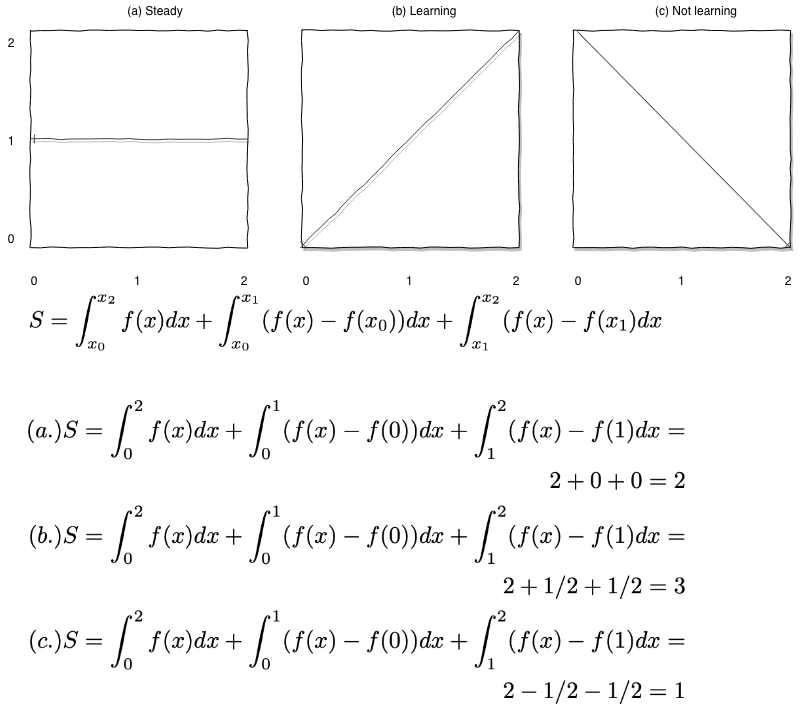
\includegraphics[keepaspectratio, width=\linewidth]{figures/fig_buschkewitheqs}
        \caption{The figure shows the computation of the \emph{Buschke Integral} scores in three scenarios. On the left figure (a) there is no learning because the subject recalls the same number of items each time ($f(x)=1, x=[0,1,2], S=2$), on the middle figure (b) the subjects learns ($f(x)=x, x=[0,1,2], S=3$) and on the right figure (c) the subject forgets items ($f(x)=2-x, x=[0,1,2], S=1$). The maximum score not (shown) is $S=4$ that corresponds with the subject recalling all the two items at each time ($f(x)=2, x=[0,1,2], S=4$).} 
        \label{fig:b}
\end{figure}

%Figure \ref{fig:b} calculates the surface of the trapezoids, it is also possible to interpolate and calculate the surface defined by the spline within the x and y axis.
One advantage of the \emph{Buschke Integral} score $S$ defined here is that it gives us a new scale of memory health condensed in one single number. This allows us to parcel the space of subjects in a larger number of meaningful categories beyond the converter versus no converter classification. The new metric upper bound is 32 (max score per trial $(16)\times (3-1)$ number of points -1) and the minimum 0.


Once we have justify the conceptual soundness of the \emph{Buschke Integral} score we need to study the clinical utility of term, to do so we will take advantage of the large dataset \emph{Vallecas Project}.

We compare the correlation between conversion to MCI and S, and single values of the Buschke test and other cognitive performance test. We also compare S with other aggregates of the Buschke test like the sum or the arithmetic and the geometric mean.

Calculate the DTW between S and a conversion or memory indicator across years, for example the ICV or the hippocampal volume. 
Plot the distribution of S $\mu = 16.37, \sigma=5.1770$, get the left tail $\mu + n*\sigma$ (worst recallers) and the right tail (best recallers) and study neurophysiological differences. Look at, hippocampal siuze, connectivity. YS: WHERE to look at

-plot the kde of bus int, use sns pairplot when i have the hippo sizes script

-correlation with conversion
- kullback leiber of distribution inter years compared with other measures (sum etc) see if distance is smaller ion. b int
- correlation with brain hippocampus

%https://kids.frontiersin.org/article/10.3389/frym.2017.00071
%https://www.scientificamerican.com/article/does-size-matter-for-brains/



\subsection{The neuroanatomy of memory}

The three main processes of memory are encoding, storage and recalling, Within recall psychologists distinguish between free recall, cue recall and serial recall.
%Ebbinghaus discovered that multiple learning, over-learning, and spacing study times increased retention of information
We own to Tulving the distinction between episodic and semantic memory, and also the encoding specificity principle which states that a person is more likely to recall information if the recall cues match or are similar to the encoding cues. 
%ojo literal wikipedia https://en.wikipedia.org/wiki/Recall_(memory)
The anterior cingulate cortex, globus pallidus, thalamus, and cerebellum show higher activation during recall than during recognition which suggests that these components of the cerebello-frontal pathway play a role in recall processes that they do not in recognition. The specific role of each of the six main regions in episodic retrieval is still unclear, but some ideas have been suggested. The right prefrontal cortex has been related to retrieval attempt;[28][29] the medial temporal lobes to conscious recollection;[30] the anterior cingulate to response selection;[31] the posterior midline region to imagery;[28][31][32][33] the inferior parietal to awareness of space;[34] and the cerebellum to self-initiated retrieval .[35]

There is a number of factors that affect recall: attention, motivation, interference, context, state-dependent memory, gender (Women perform better than males on episodic memory tasks including delayed recall and recognition. However, males and females do not differ on working, immediate and semantic memory tasks.) physical activities





%ojo +-lit from margolin1992cognitive
Many years ago Lashley \cite{lashley1929brain} set out to find the engram the putative site of memory storage and his failure toi find a specific location (in rats) led him to the conclussion that memories were spatially distributed  throughout the brain. Squire \cite{squire2004memory} pointed out to methodological shortcoming in Lashley's work but in general terms his conclusions are considered valid.
One suggestion is thet engrams are stored in cerebral cortex near the regions where the stimuli is processed eg visual memories near occipìtal, auditory components in auditory cortex and so for. 
By exclusion (HM) we know that the memory abilities preserved by amnesic subjects would not be dependent of removed areas (hippocampus, or medial dorsal nucleus). Habit formation is known to be mediated by the amygdala, conditioning of motor responses in the basal ganglia and working memory to frontal and parietal regions \cite{margolin1992cognitive} pg. 178. 


Amnesia or memory disorders can be grouped in terms of etiology or in terms of neuroanatomy. The former we can mention AD, anoxia, etc.In terms of neuroanatomy some have distinguished between hippocampal and diancephlic amnesia (mammalian bodies and or thalamus)
Where are memories stored in the brain? Broadly speaking a classification can be made:

How to assess memory performance?
\begin{itemize}
\item Assessment of Explicit or episodic memories 
\begin{itemize}
  \item Wechsler memory scale(WMS) it has been critizied
  \item Buschke Selective Reminding Procedure, more sophisticated than WMS, the subject attempts to learn a list a word list across several (3) trials. It allows generation of a variety of scores (sum recall, LTretrieval, ST retrieval ...). The popularity resides in the reduced testing time, word list learning may be better than story recall and separation between retrieval and enter in formation into long term store. Among the criticism is the B. is more a procedure than a test per se (the word list, number of words and number of trials vary widely). Furthermore, B assumes that if a subject fails to to recall a word that has been previosuly recalled in LTM the retrieval failure is a recall failure
\end{itemize}  
\item Explicit or Implicit memories (preserved in amnesia)
\begin{itemize}
\item  Sentence puzzle completion
\end{itemize}
\end{itemize}  
There are many issues that the memory test assessment elude, for example Metamemory and confabulation. Metamemory is the knowledge one posses about the functioning of the human memory system (for example, if one is using Anki (Hermann Ebbinghaus theory of retention training)). Confabulation is poorly understood, intrusions on list learning may be related to confabulation.

%https://qbi.uq.edu.au/brain-basics/memory/where-are-memories-stored
\begin{itemize}
\item Explicit declarative or episodic memories and semantic memories: hippocampus, neocortex and amygdala.
\begin{itemize}
  \item Hippocampus is part of the temporal lobe and is where explicit or episodic memories are formed and indexed for later access. (we know this thanks to Henry Molaison who had his medial temporal lobe (hippocampus, amygdala, and enthorinal cortex) surgically removed to treat his epilepsy, rendering him amnesic but with capacity to learn motor tasks)
  \item Neocrotex is the neural tissue that forms the outside surface of the brain. Transfer from the hippocampus (temporary) to the neocortex (general knowledge) may happen during sleep
  \item Amygdala is an almond shape structure above the hippocampus and attaches emotional significance to memories, this is why memories associated with grief , shame etc are difficult to forget, characterizing the path amygdala, hippocampus, neocortex may explain how memories are retained. The amygdala not only adds strength to the emotional memory, it also plays a role in forming new memories, specially related to fear. Fearful memories are able to be formed after a few repetitions
\end{itemize} 
\item Implicit memories (eg motor) cerebellum and basal ganglia
\begin{itemize}
  \item cerebellum located at the rear base of the brain, important in motor control eg the vestibulo-ocular reflex let us maintain our gaze on a location as we rotate our heads.
  \item Basal ganglia lying deep within the brain and involved in habit formation, reward processing and learning. They co-ordinate sequences of motor activity, it is the most affected region in Parkinson's. disease
\end{itemize}
\item Short-term working memory prefrontal cortex
\begin{itemize}
  \item Prefrontal cortex seats at the very front of the brain and it is the most recent addiction to the mammalian brain, holding information activates the pFC, there seems to exist a functional separation between left and right sides of the pFC.
\end{itemize}  
\end{itemize}

Note that another classification of memories is Long term memories including Explicit and Implicit and short term memories. Short term (primary or active memory) is the capacity for holding, but not manipulating, a small amount of information in mind in an active, readily available state for a short period of time.  The duration of short-term memory (when rehearsal or active maintenance is prevented) is believed to be in the order of seconds (Miller's law magical number 7 +-2 and more recently Cowan 4+-1.).
The modal model of memory was developed in the 1960s by Shiffrin and assumed that all memories pass from a short-term to a long-term store after a small period of time. The exact meachanisms by which this transfer occurs is unclear.

One evidence of the existence of short-term store comes from anteroretrogade amnesia which is the inability to learn new facts and episodes, patients with this amnesia (eg HM) have intact its ability to retain small amounts of information over small time scales (30 seconds) but are unable to form long term memories. Other evidence comes from distraction interventions, a distraction may impair memory 3-5 most recently learned words of a list (to be stored in short  term memory) while leaving the recall for words earlier in the list intact (to be stored in long term memory). See, however, \cite{bjork1974recency}, for a criticism of the existence of short term memory using a distractor task. But not everyone agrees that short and long term memories vary independently, the unitary model states that memory is unitary over time scales from milliseconds to years. Admittedly it has been difficult to demarcate the a clear boundary between short and long term memories.

The biological basis STM: stimuli are coded in STM using transmitter depletion, the stimulus activates a spatial pattern of neurons and as they fire they deplete the available neurotransmitters, the pattern of depletion is iconic (WOW!) representing the stimulus functioning as a memory trace. As the neurotransmitters reuptake mechanisms kick in to restore the pre stimulus level, the memory trace decays \cite{grossberg1971pavlovian}.

\begin{figure}[H]
        \centering
        \includegraphics[keepaspectratio, width=.5\linewidth]{figures/memory_types}
        \caption{Memory types under the modal or multi-store or Atkinson-Shiffrin model. Alternatively, the Fergus Craik and Robert Lockhart in 1972, and posits that memory recall, is a function of the depth of mental processing, on a continuous scale from shallow (perceptual) to deep (semantic). Under this model, there is no real structure to memory and no distinction between short-term and long-term memory. Anothe classification is the to Multiple Trace Theory, long-term episodic memories are stored in hippocampus, so mild AD patients, even MCI, will lose these kind of "long-term" memories. Long term semantic memories will be lost in parallel with neocortex neuron death.
        %http://www.human-memory.net/types.html
        } 
        \label{fig:b}
\end{figure}

%Rehearsal is the process where information is kept in short-term memory by mentally repeating it. When the information is repeated each time, that information is reentered into the short-term memory, thus keeping that information for another 10 to 20 seconds (the average storage time for short-term memory)
\newpage
\addcontentsline{toc}{section}{References}


% BibTeX users please use
\bibliographystyle{apalike}
\bibliography{../bibliography-jgr/bibliojgr}



\end{document}